
\section{Decision Variable Scalability Studies}
\IEEEPARstart{}{} The scalability study is carry out with the configuration established in the section IV.
%
In addition, others instances are carefully selected based in their properties, therefore some problems can be easily approximated to the Pareto front with long term executions.
%
In the first place, considered as an easy problem is the DTLZ4, which is separable-unimodal and the Pareto shape is concave, also it has a polynomial bias.
%
In the same way, considered more difficult than DTLZ4 are DTLZ7 and WFG2, due that each one has multiple optimums, also these problems are separable and non-separable respectively. 
%
Thereafter, the WFG8 is considered as more difficult problem than previously mentioned, due that it has a high parameter dependence.
%
In contrast, the UF problems are popularly hard in the MOEAs and specifically are conformed of two and three objectives, these problems were proposed in CEC-2009 \cite{Joel:CEC2009}.
%
Particularly, in this work are chosen the UF5, UF7 and UF10, where the first pair are conformed with two objectives and the last one consist of three objectives.
%

As is showed empirically in the figures \ref{tab:StatisticsHV_2obj} and \ref{tab:StatisticsHV_3obj}, the VSD-MOEA proves to be very stable, although that in the DTLZ7 with two objectives is improved by the GDE3.
%
However the GDE3 is affected in difficult instances as are UF5, UF10, WFG2 and WFG8, also with three objectives it is seriously deteriorated.
%
Additionally, as it is explained in \cite{Joel:GDE3_CEC09} the DE operators can be aggressive inducing diversity issues in long term executions resulting in an unstable development 	related with their parametrization .
%
Equally important is to mention the effect of MOEA/D and MOMBI-II with three objectives, due that these algorithms are guided by weight vectors, therefore is expected a degree of stability, nevertheless if some regions are not reached, then the performance is compromised as occurs with multiple optimal regions.
%
Also some figures shows a small improvement when more variables are considered, specifically this could occurs due that the decision space involved is higher and provokes more diversity in the solutions, therefore in some situations locate better solutions.

\section{Influence Study of Parameter $D_I$}

Principally, the diversity is influenced in the VSD-MOEA through the parameter $D_I$, which is explained in the section III, where is indicated that this parameter is computed through the formula $D_I = k * \sqrt[]{N}  \rightarrow k \in (0,1)$ where $N$ is the dimension of the decision variable pace.
%
The effect of the parameter $k$ is illustrated in the figure \ref{fig:Tuning}, each graph represents the hypervolume average through 35 executions of each initial parameter $k = \{ 0.0, 0.1, 0.2, 0.3, 0.4, 0.5, 0.6, 0.9 \}$, it is important to take into account that the diversity is not promoted in the case of the assignment $k= 0.0$, therefore in difficult instances this value should provide low hypervolume values. 
%
In some instances as WFG9 the HV is deteriorated according increases the parameter $k$, this occurs due that these problems are easily approximated, thus in all the time execution the solutions are better located in the objective space and therefore the period of time induced in the first phase (diversity promoting) is wasted.
%
However this issue can be solved through a local search being part of the second phase of the total execution.
%
In general, it seems that the algorithm is enough stable, given that different values of $k$ does not provide drastically differences in the solutions.

\begin{figure*}[t]
\centering
\caption{Tuning study of parameter $k$ }
\label{fig:Tuning}
\begin{tabular}{ccc}
\includegraphics[width=0.22\textwidth, angle=-90,origin=c]{Tuning/2obj_DTLZ4.eps} &
\includegraphics[width=0.22\textwidth, angle=-90,origin=c]{Tuning/2obj_DTLZ7.eps} &
\includegraphics[width=0.22\textwidth, angle=-90,origin=c]{Tuning/2obj_WFG8.eps} \\
\includegraphics[width=0.22\textwidth, angle=-90,origin=c]{Tuning/3obj_DTLZ4.eps} &
\includegraphics[width=0.22\textwidth, angle=-90,origin=c]{Tuning/3obj_DTLZ7.eps} &
\includegraphics[width=0.22\textwidth, angle=-90,origin=c]{Tuning/3obj_WFG8.eps} \\
\includegraphics[width=0.22\textwidth, angle=-90,origin=c]{Tuning/2obj_WFG9.eps} &
\includegraphics[width=0.22\textwidth, angle=-90,origin=c]{Tuning/UF5.eps} &
\includegraphics[width=0.22\textwidth, angle=-90,origin=c]{Tuning/UF6.eps} \\
\includegraphics[width=0.22\textwidth, angle=-90,origin=c]{Tuning/3obj_WFG9.eps} &
\includegraphics[width=0.22\textwidth, angle=-90,origin=c]{Tuning/UF8.eps} &
\includegraphics[width=0.22\textwidth, angle=-90,origin=c]{Tuning/UF10.eps} 
\end{tabular}
\end{figure*}



\section{Attainment Surfaces}

The 50\% attainment surfaces achieved of some two objective instances are showed in the figure \ref{fig:Attainment_Surfaces}, the rest of instances are not significantly different by all the algorithms, therefore are not attached in this document.
%
The more significant improvements are showed in the instances DTLZ7, WFG2, WFG8 and UF5, where the VSD-MOEA locate solutions in regions that are not reached by the rest of algorithms.
%
Although the GDE3 approximates the Pareto front adequately as the VSD-MOEA in some problems, in the WFG8 and WFG9 the GDE3 has a poor performance, therefore it confirms the DE diversity issues.
%
Accordingly, based in this development and under this situation the genetic operator can be considered more robust than the basic operators of differential evolution.



\section{Statistics with Inverted Generational Distance Plus}

The IGD+ is a metric considered weakly Pareto compliant \cite{Joel:Inverted_Generational_Distance_Plus}, it qualify the convergence and diversity of no-dominated solutions obtained along the Pareto front.
%
However there exist the inconvenient, this metric needs a set of reference points well distributed that belong to the Pareto front.
%
Particularly, this is a inconvenient with some benchmark, e.g. the WFG problems due these problems do not have the Pareto front in a fixed location, since it depends of the distance and position parameters of the decision variables and although the WFG authors provide a generator of solutions, still exist a problem generating the reference points in some problem with bias issues. 
%
To deal with this inconvenient, the process consist in the next steps. First, the difficulties are removed of each instance generating a number of solutions (in this case 10000), thereafter the close solutions are removed through a specific cluster method .

%
The statistical test of two and three objectives are showed in the tables \ref{tab:StatisticsHV_2obj} and \ref{tab:StatisticsHV_3obj} respectively.
%
In particular with two objectives the VSD-MOEA and GDE3 have the best means, however the VSD-MOEA has a lowest average Diff value than GDE3, therefore our proposal does not provide significantly poor values in any instance, in fact the worst are the DTLZ6 and UF3.
%
In the same way, considering three objectives the GDE3 is severely compromised, however the VSD-MOEA maintain low IGD+ values, in fact it still has the lowest Diff value, also as could be expected the MOMBI-II provides low mean values in some instances, specifically this occurs due that this algorithm is based in predefined weight vectors.
%

On the other hand, the effective tests are showed in the tables \ref{tab:Effective_Test_2obj} and \ref{tab:Effective_Test_3obj}, as is explained in the section IV these metrics qualify the superiority of each algorithm with the rest through pair comparisons.
%
The VSD-MOEA provides the best scores considering two objectives, in the second place is the GDE3, however it is deteriorated with three objectives, also it has high negative scores.
%
Principally, in three objectives case VSD-MOEA not only provide the best general score, but also duplicates the second best score that belong to the state-of-art (VSD-MOEA with $10.16$ and MOMBI-II with $4.763$).
%
Moreover the VSD-MOEA provides the best scores with the majority of the difficult instances or is enough close that the best values.
%
Finally, it is important to take into account that our proposal does not provides high negative scores with two objectives and get better with three objectives.
%
Therefore this can be a clue that this principle can be applied with many-objective problems.

%%%%%%ESTUDIO DE ESCALABILIDAD

\begin{figure*}[h]
\centering
\caption{Scalability study of decision variables with two objectives (HV)}
\label{fig:Scalability_Study_HV_1}
\begin{tabular}{ccc}
   \includegraphics[width=0.23\textwidth, angle=-90,origin=c]{Images/DTLZ4_2obj_Scalability.eps} &
    \includegraphics[width=0.23\textwidth, angle=-90,origin=c]{Images/DTLZ7_2obj_Scalability.eps} &
    \includegraphics[width=0.23\textwidth,  angle=-90,origin=c]{Images/UF7_Scalability.eps}  
    \\
   \includegraphics[width=0.23\textwidth, angle=-90,origin=c]{Images/UF5_Scalability.eps} &
   \includegraphics[width=0.23\textwidth, angle=-90,origin=c]{Images/WFG2_2obj_Scalability.eps} &
   \includegraphics[width=0.23\textwidth, angle=-90,origin=c]{Images/WFG8_2obj_Scalability.eps}  
\end{tabular}
\end{figure*}

\begin{figure*}[h]
\centering
\caption{Scalability study of decision variables with three objectives (HV)}
\label{fig:Scalability_Study_HV_1}
\begin{tabular}{ccc}
\includegraphics[width=0.23\textwidth, angle=-90,origin=c]{Images/DTLZ4_3obj_Scalability.eps} &
\includegraphics[width=0.23\textwidth, angle=-90,origin=c]{Images/DTLZ7_3obj_Scalability.eps} &
\includegraphics[width=0.23\textwidth, angle=-90,origin=c]{Images/UF10_Scalability.eps}  
\\
 \includegraphics[width=0.23\textwidth, angle=-90,origin=c]{Images/WFG2_3obj_Scalability.eps} &
  \includegraphics[width=0.23\textwidth,   angle=-90,origin=c]{Images/WFG8_3obj_Scalability.eps}  
\end{tabular}
\end{figure*}
%%%%%%%%%%%SUPERFICIES DE CUBRIMIENTO LOGRADAS

\begin{figure*}[h]
\centering
\caption{50\% Attainment Surfaces Achieved}
\label{fig:Attainment_Surfaces}
\begin{tabular}{ccc}
%  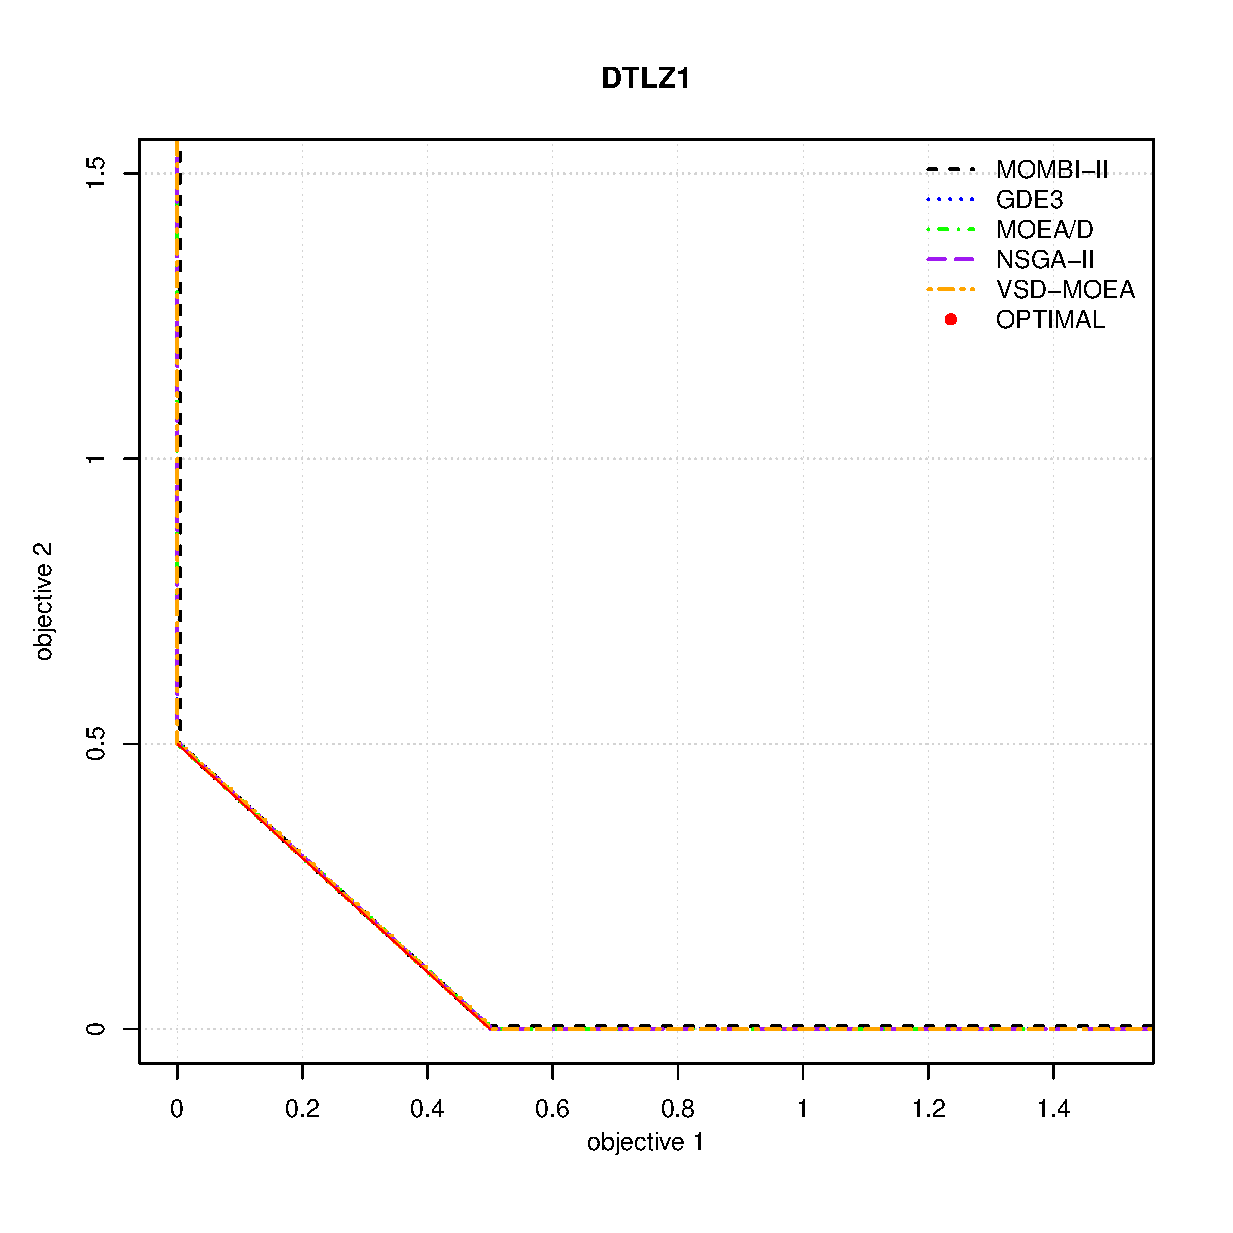
\includegraphics[width=0.33\textwidth]{Surfaces/DTLZ1.eps} &
  %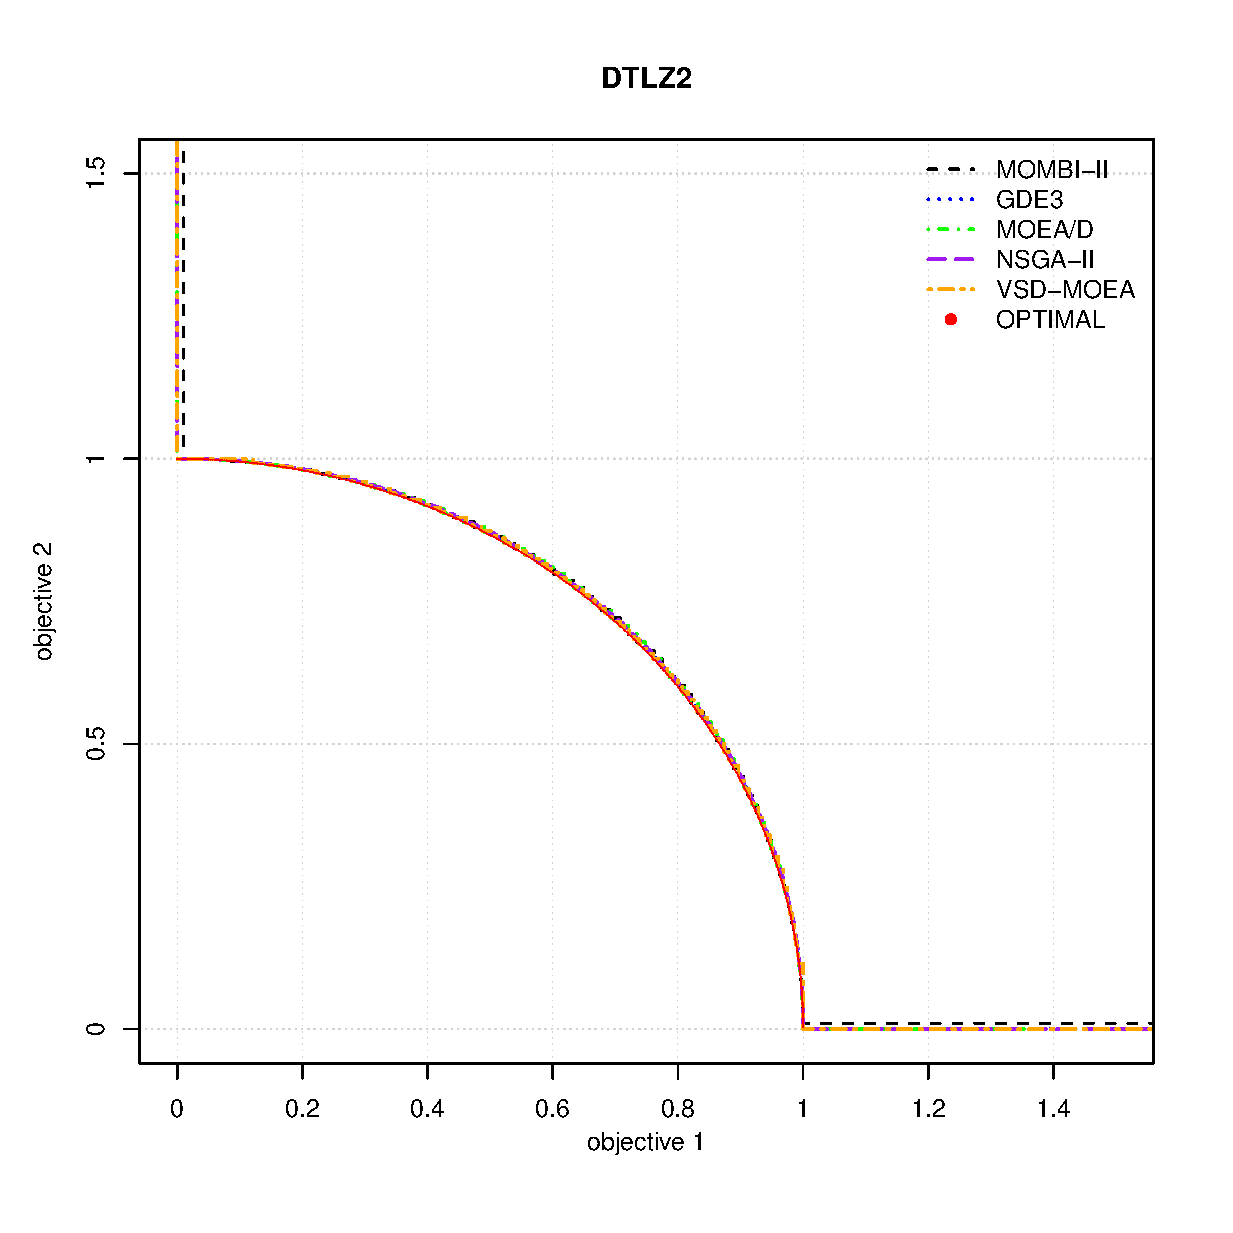
\includegraphics[width=0.33\textwidth]{Surfaces/DTLZ2.eps} &
  %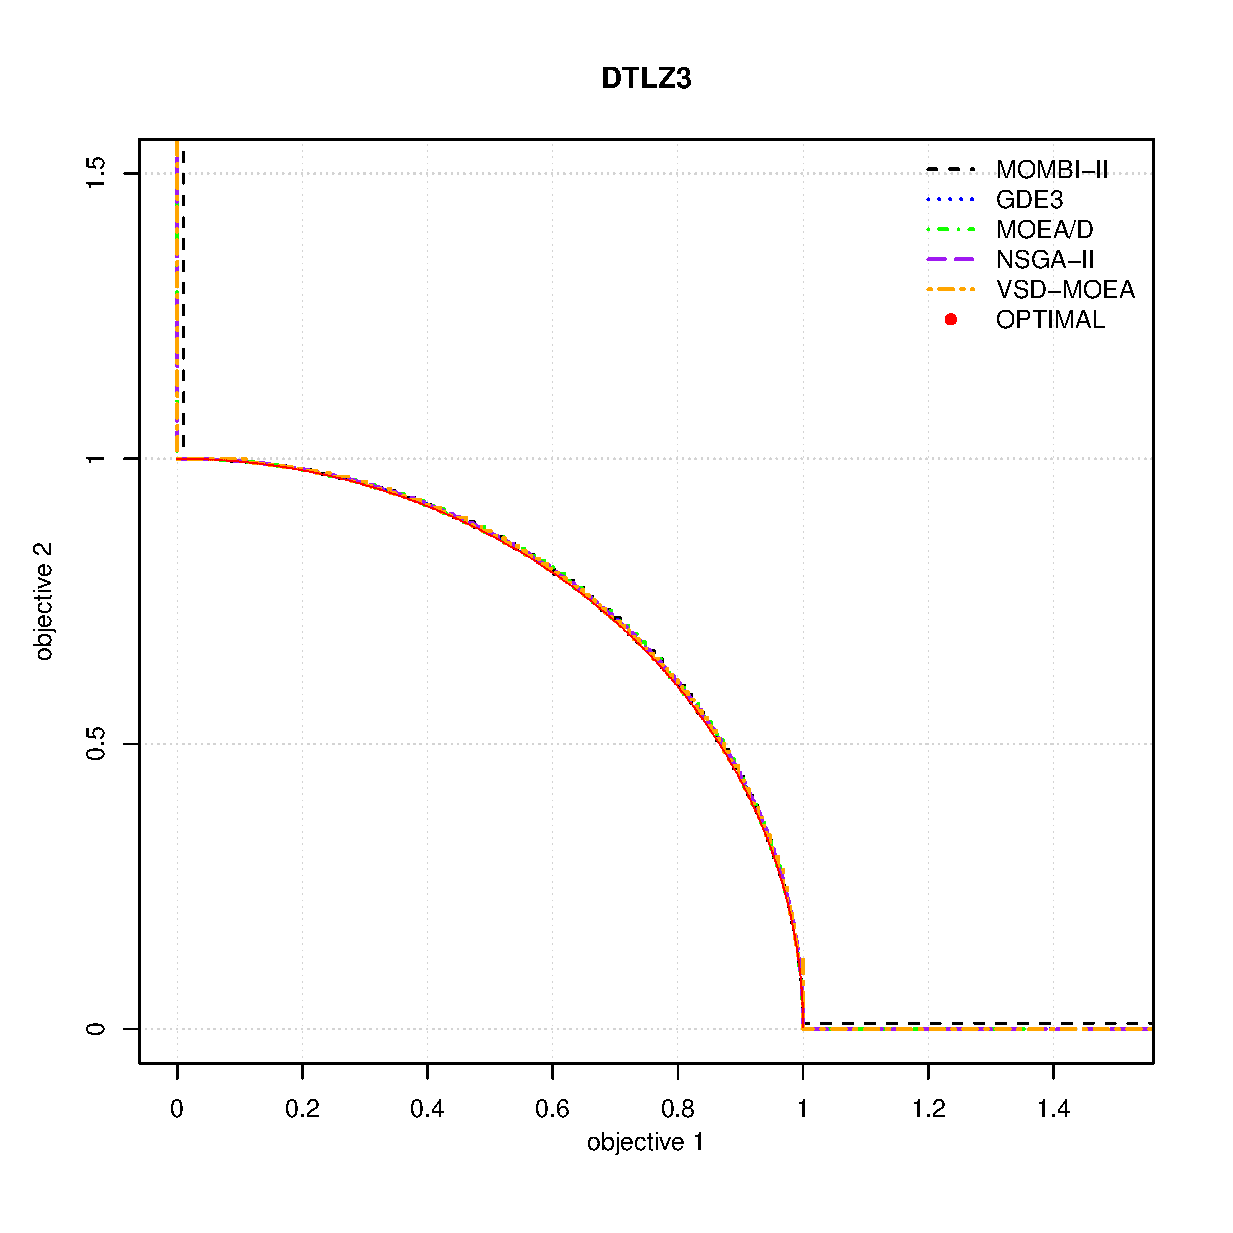
\includegraphics[width=0.33\textwidth]{Surfaces/DTLZ3.eps} \\
  %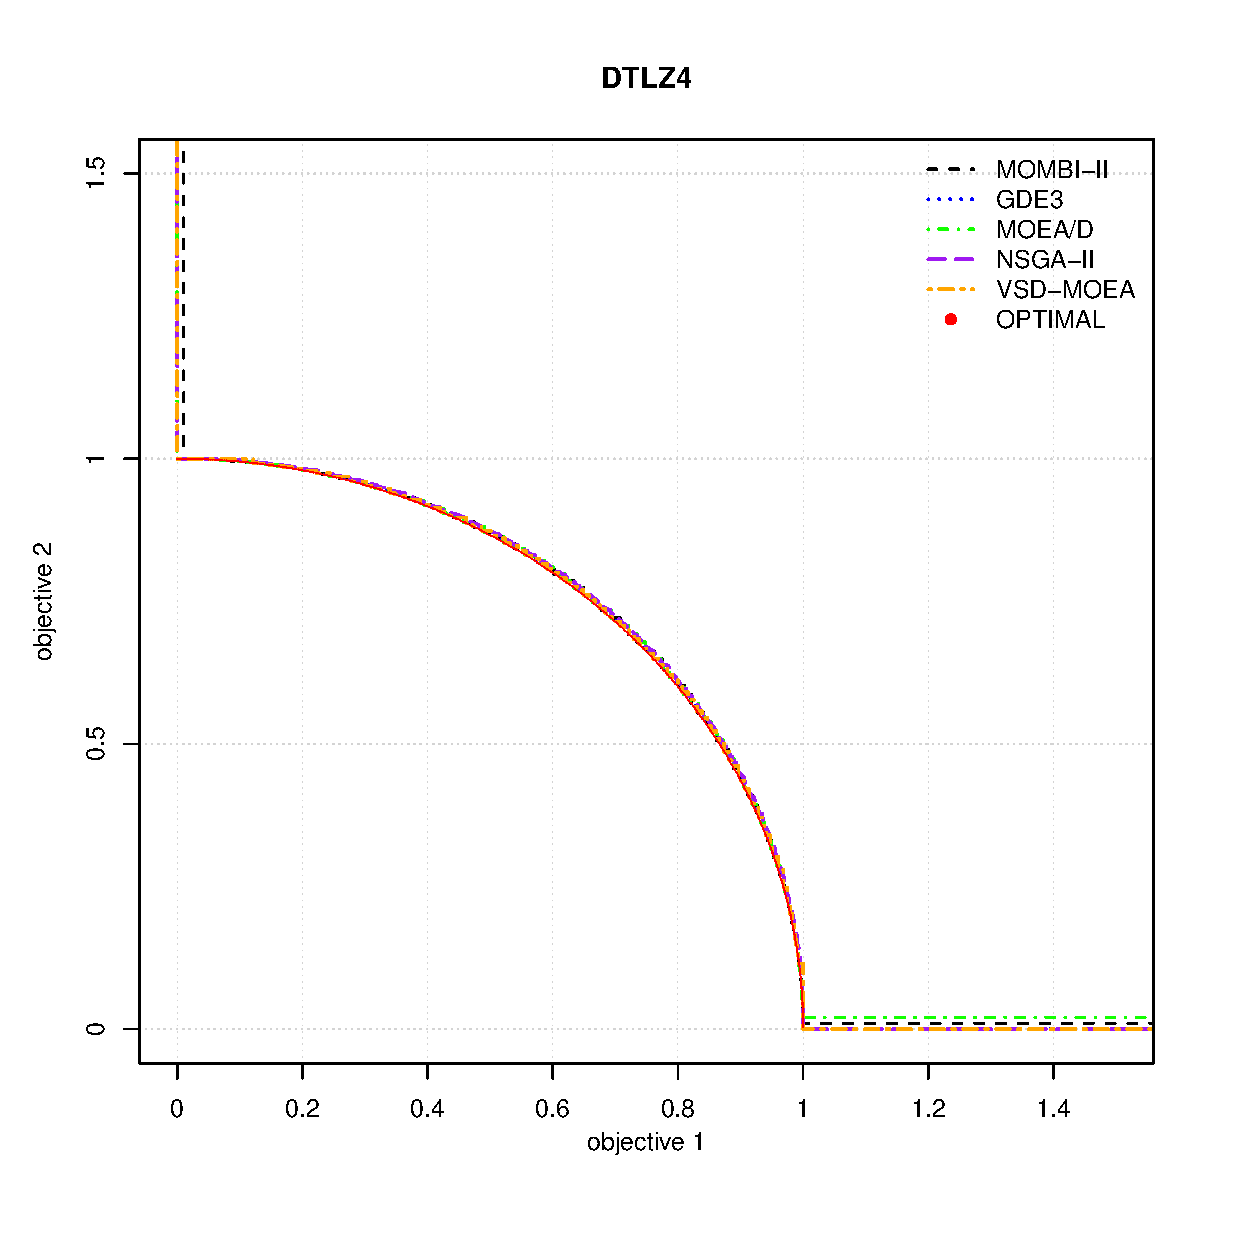
\includegraphics[width=0.33\textwidth]{Surfaces/DTLZ4.eps} &
  %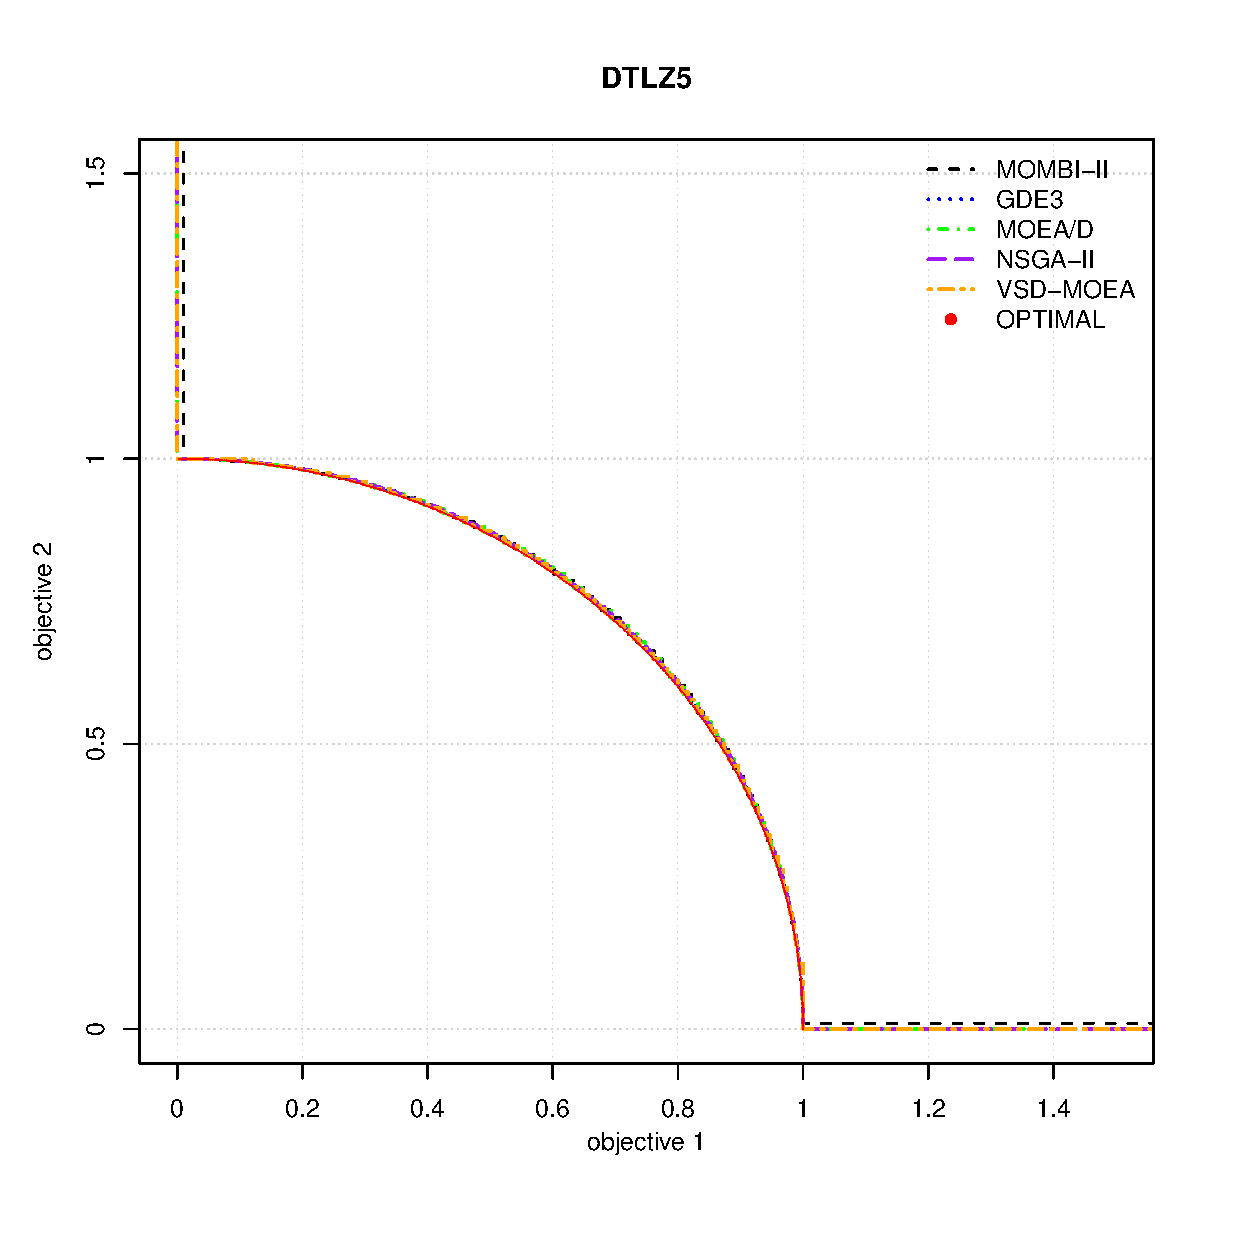
\includegraphics[width=0.33\textwidth]{Surfaces/DTLZ5.eps} &
  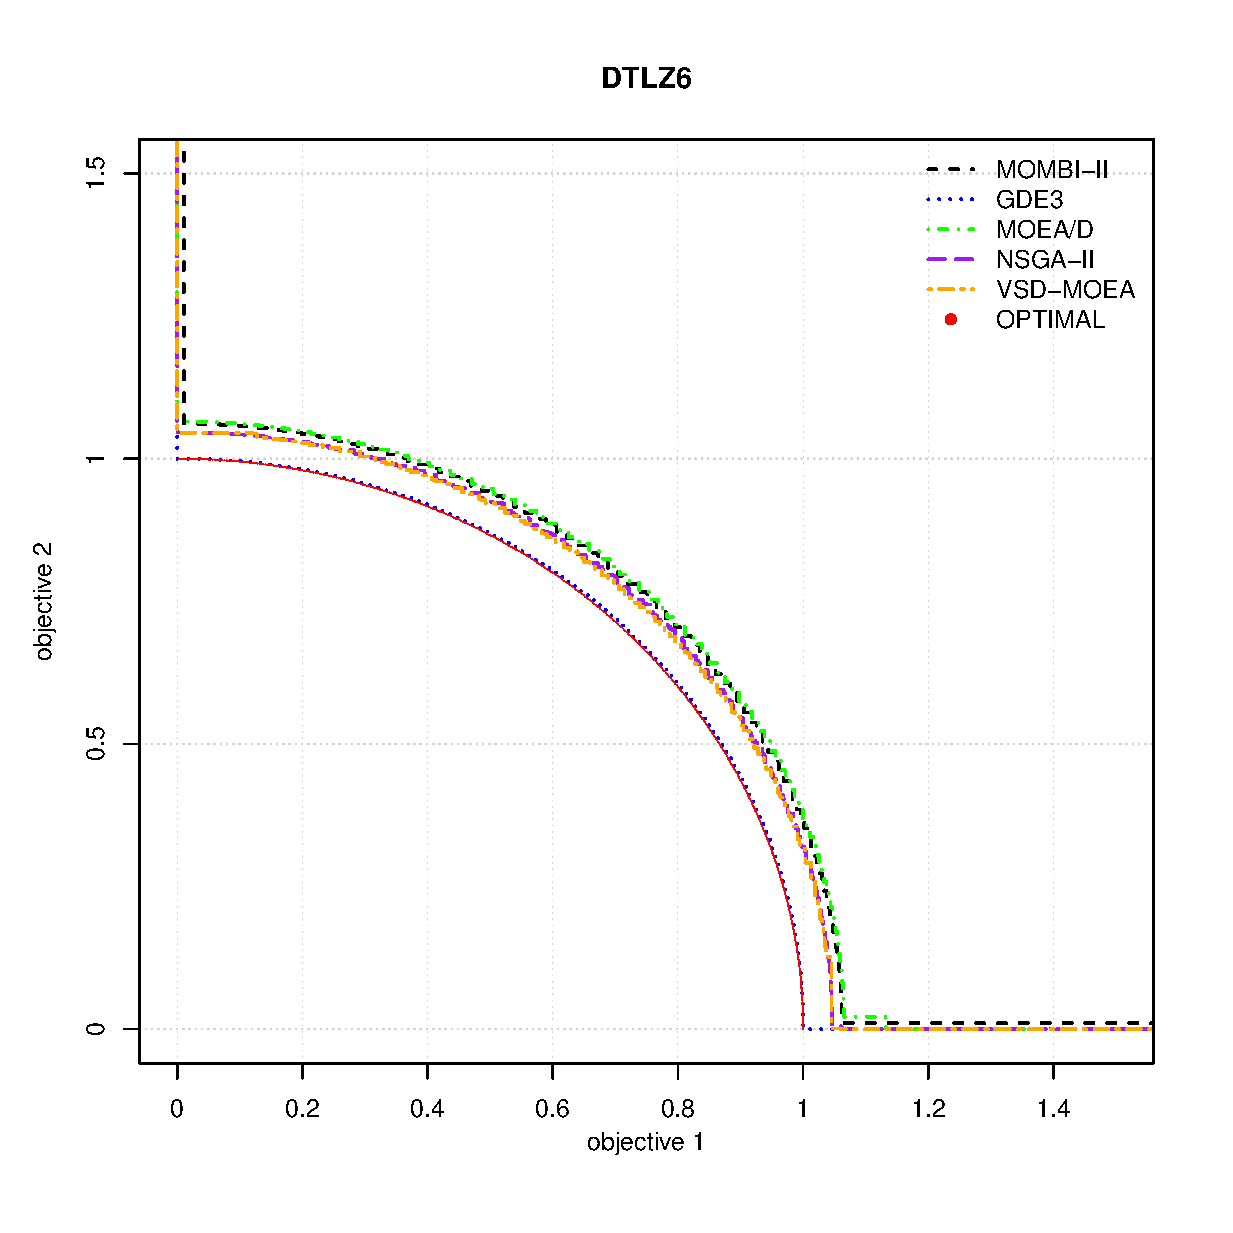
\includegraphics[width=0.33\textwidth]{Surfaces/DTLZ6.eps} &
  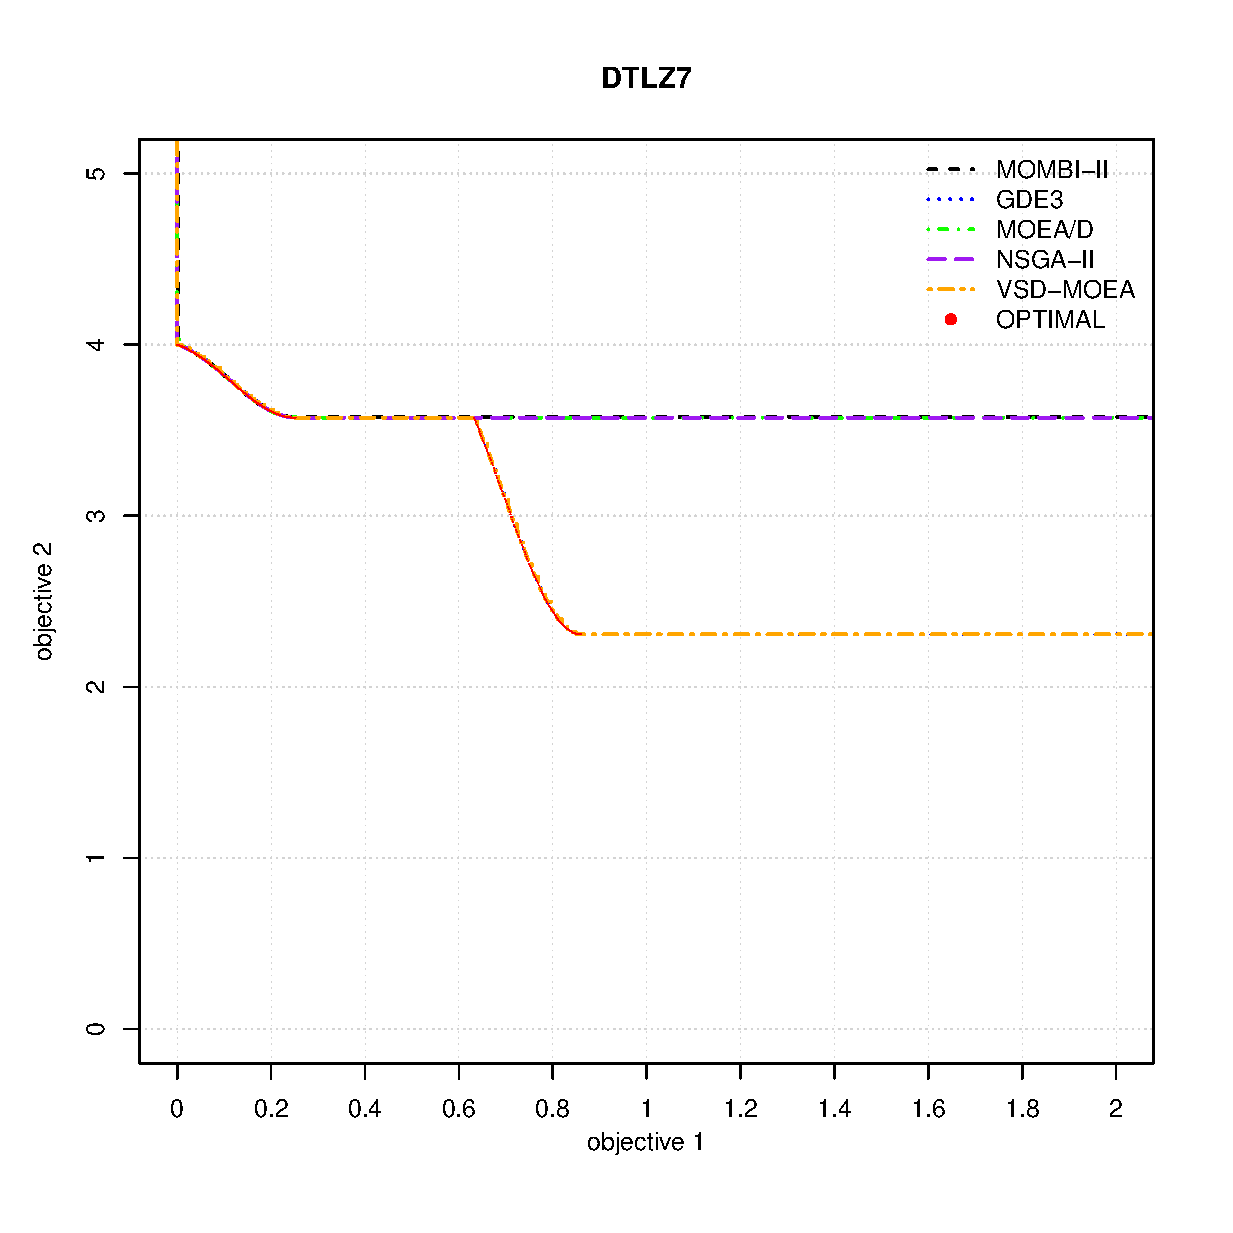
\includegraphics[width=0.33\textwidth]{Surfaces/DTLZ7.eps} &
%   \end{tabular}
% \end{figure*}
 
%  \begin{figure*}
% \centering
% \caption{50\% Attainment Surfaces Achieved}
% \begin{tabular}{ccc}
  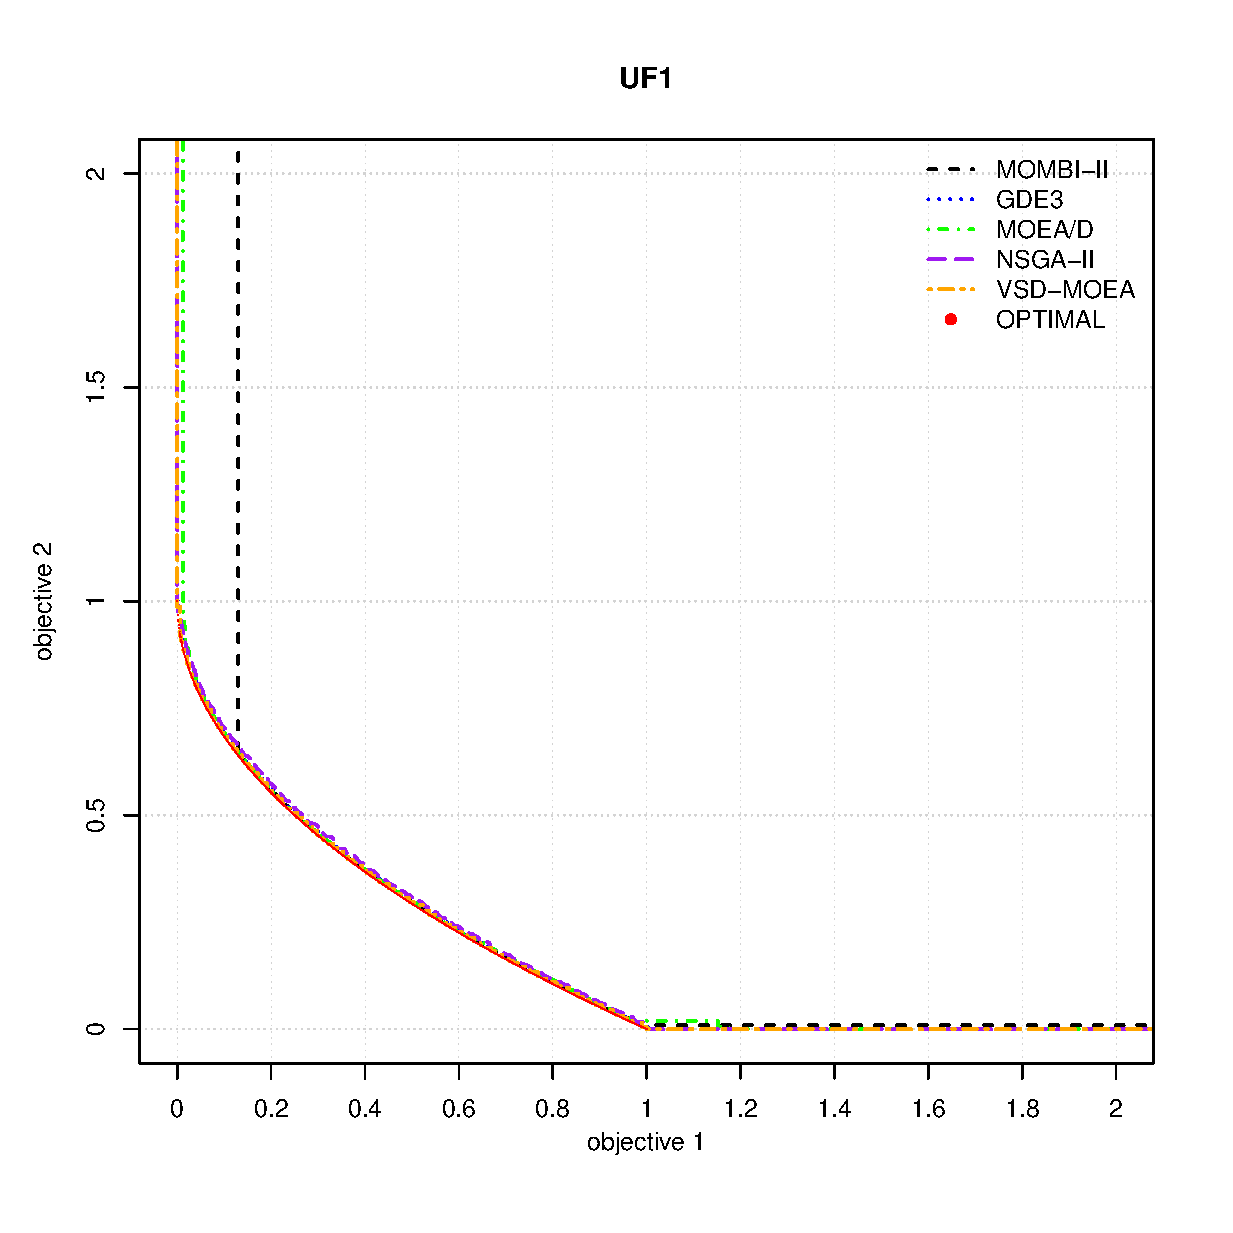
\includegraphics[width=0.33\textwidth]{Surfaces/UF1.eps} 
  \\
  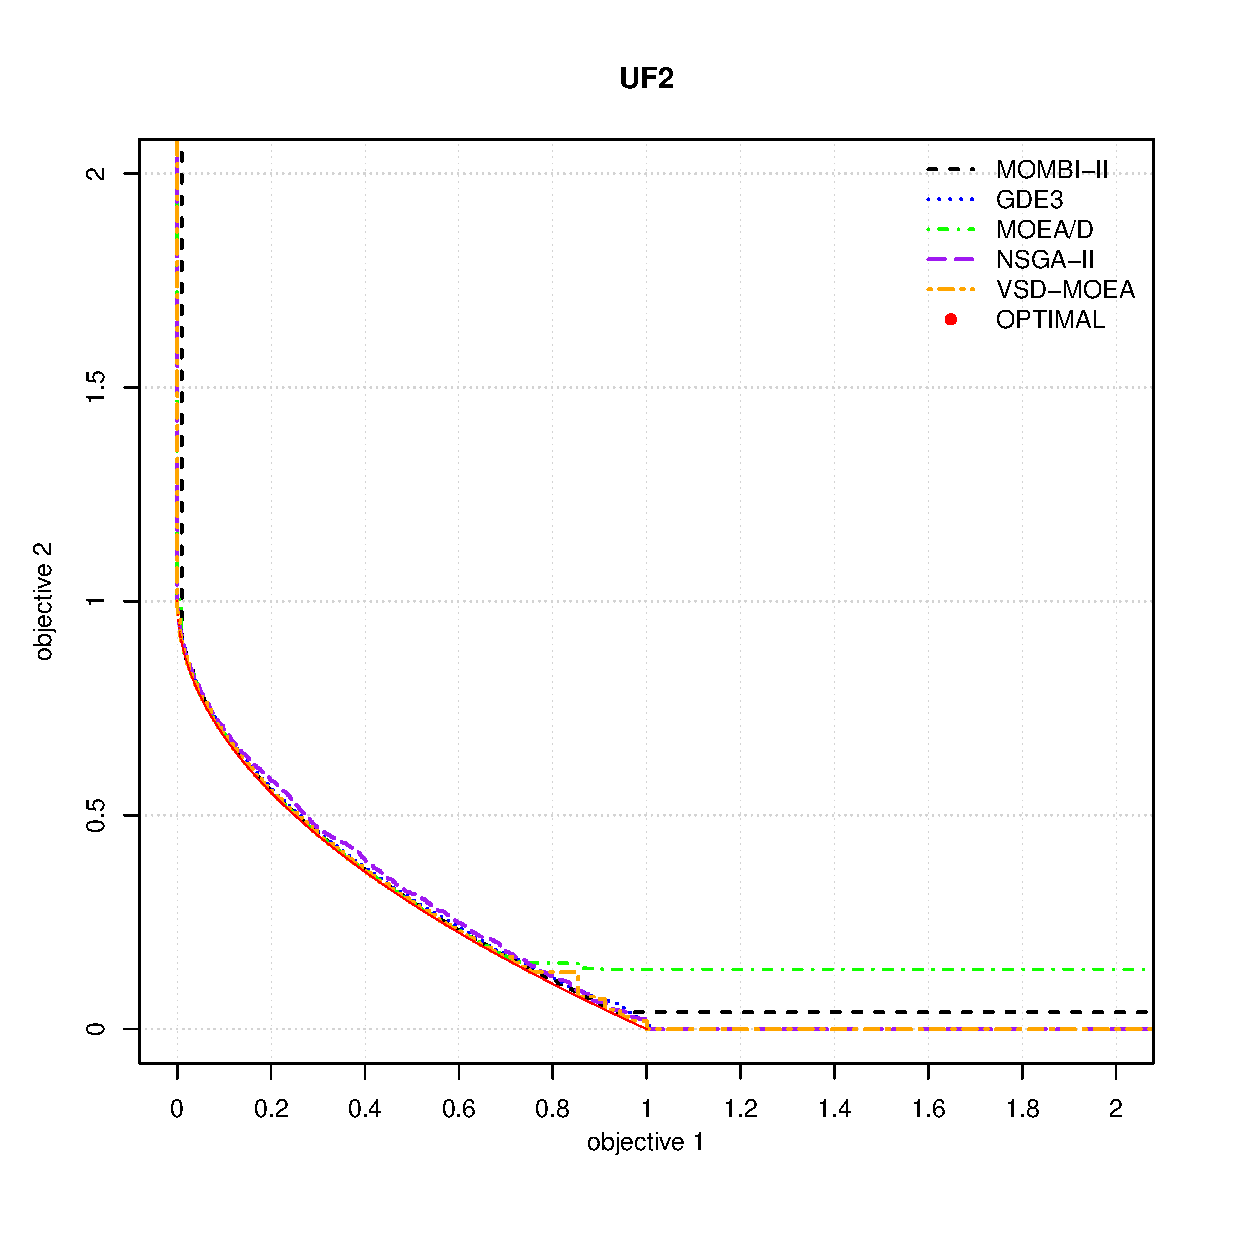
\includegraphics[width=0.33\textwidth]{Surfaces/UF2.eps} &
%  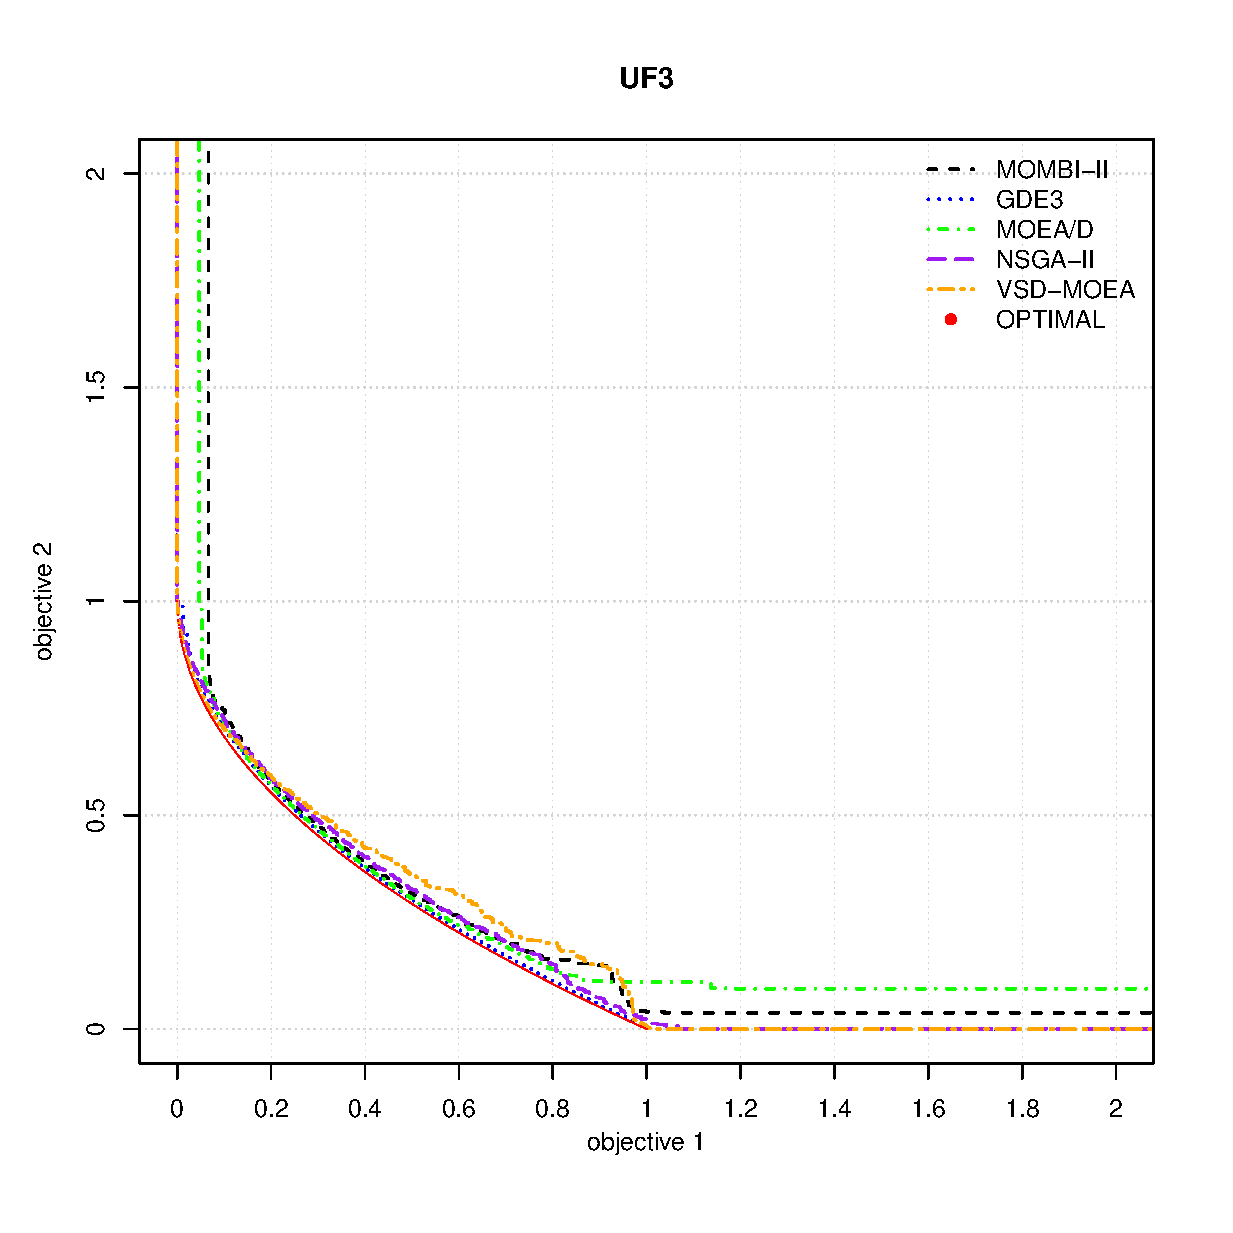
\includegraphics[width=0.33\textwidth]{Surfaces/UF3.eps} &
  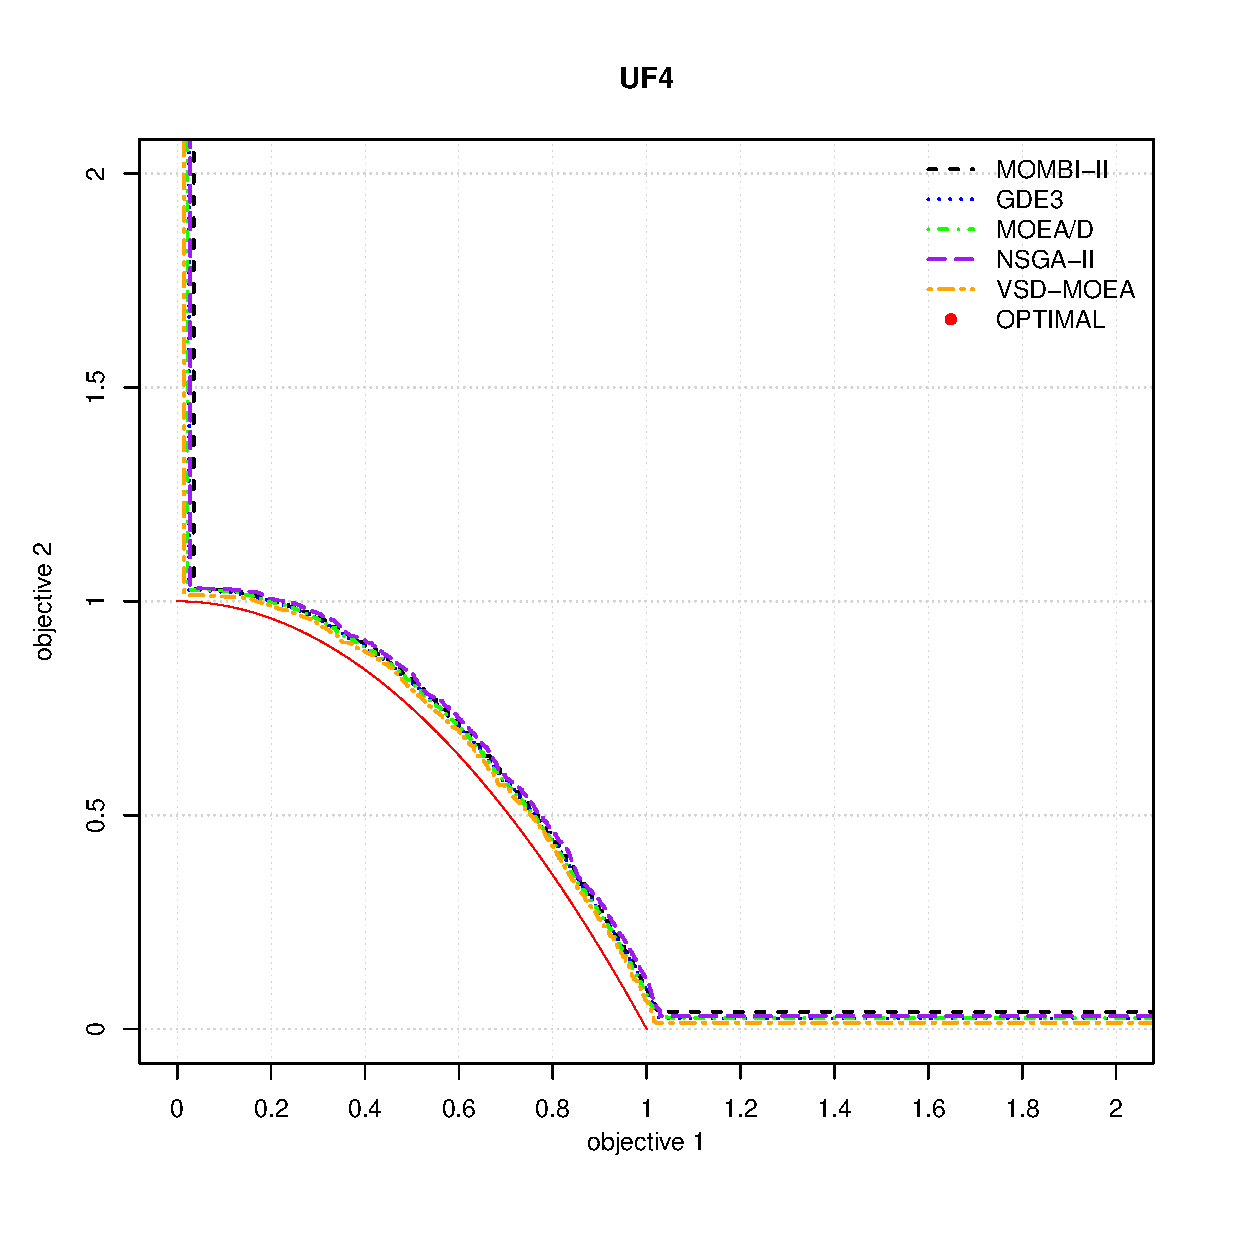
\includegraphics[width=0.33\textwidth]{Surfaces/UF4.eps} &
  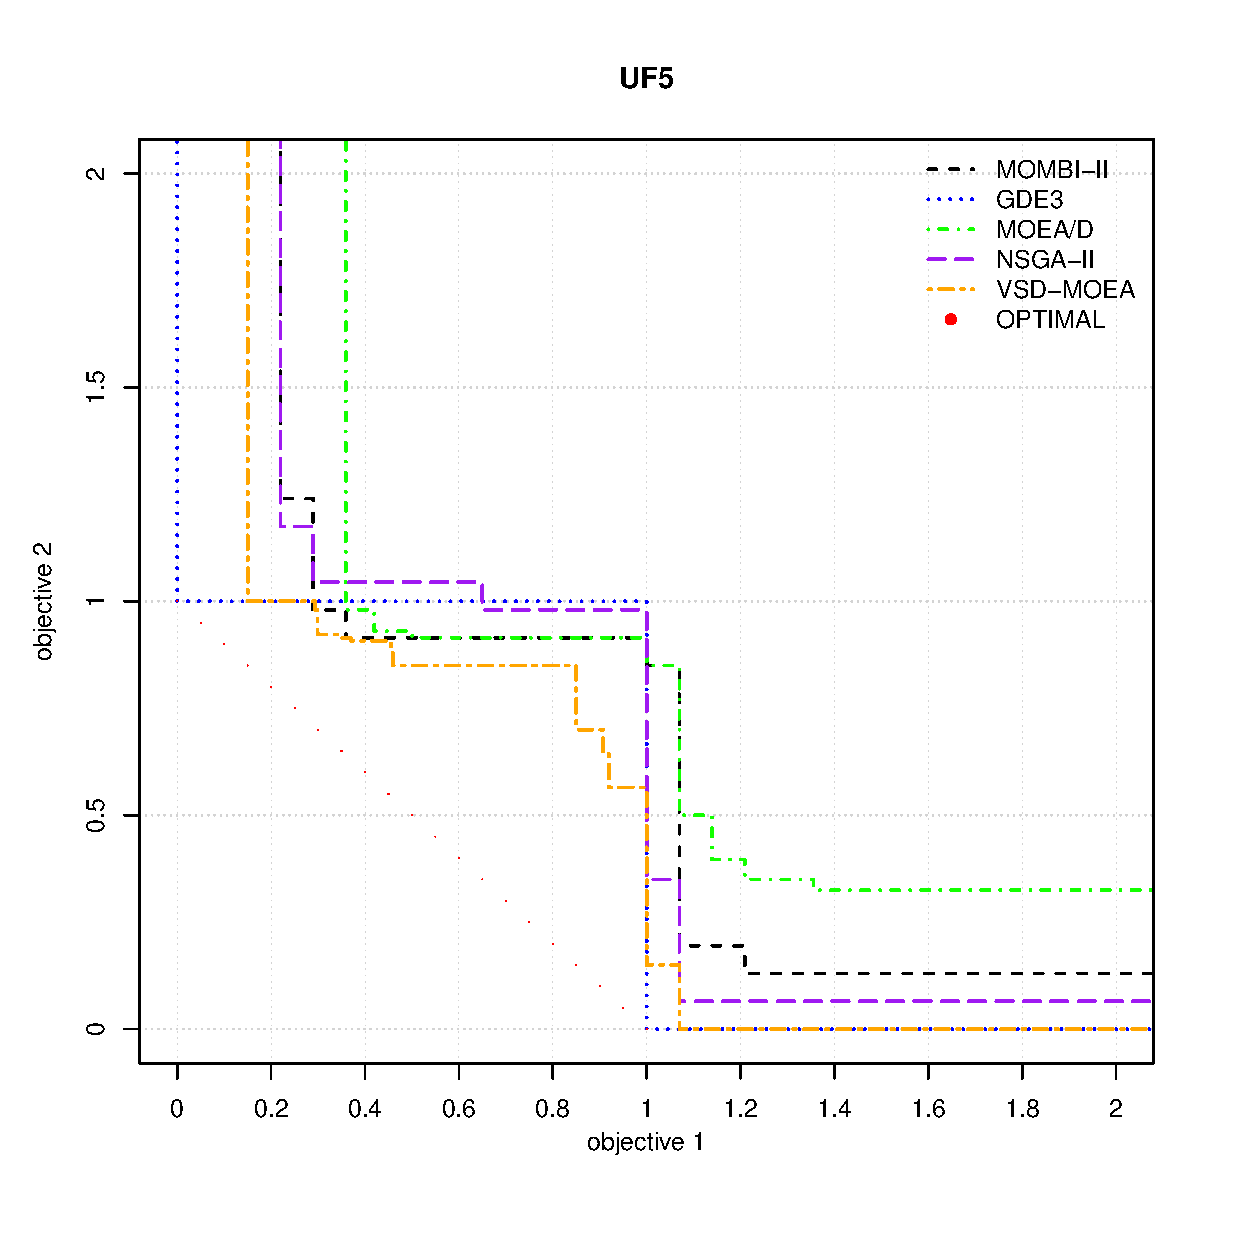
\includegraphics[width=0.33\textwidth]{Surfaces/UF5.eps}  
  \\
  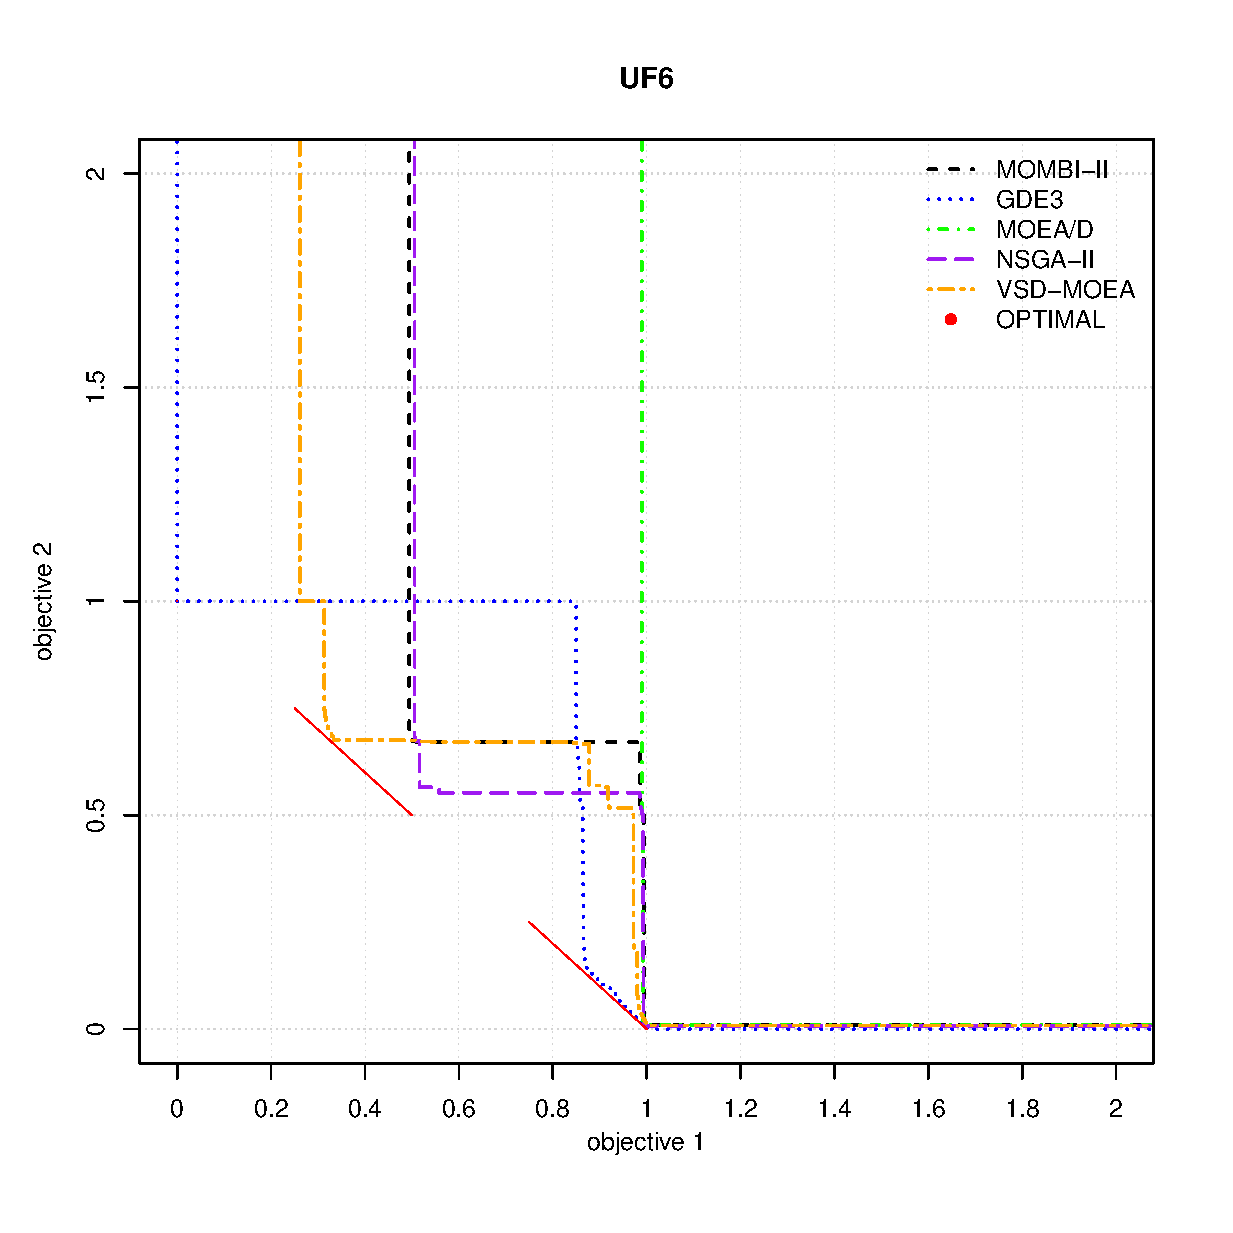
\includegraphics[width=0.33\textwidth]{Surfaces/UF6.eps} &
  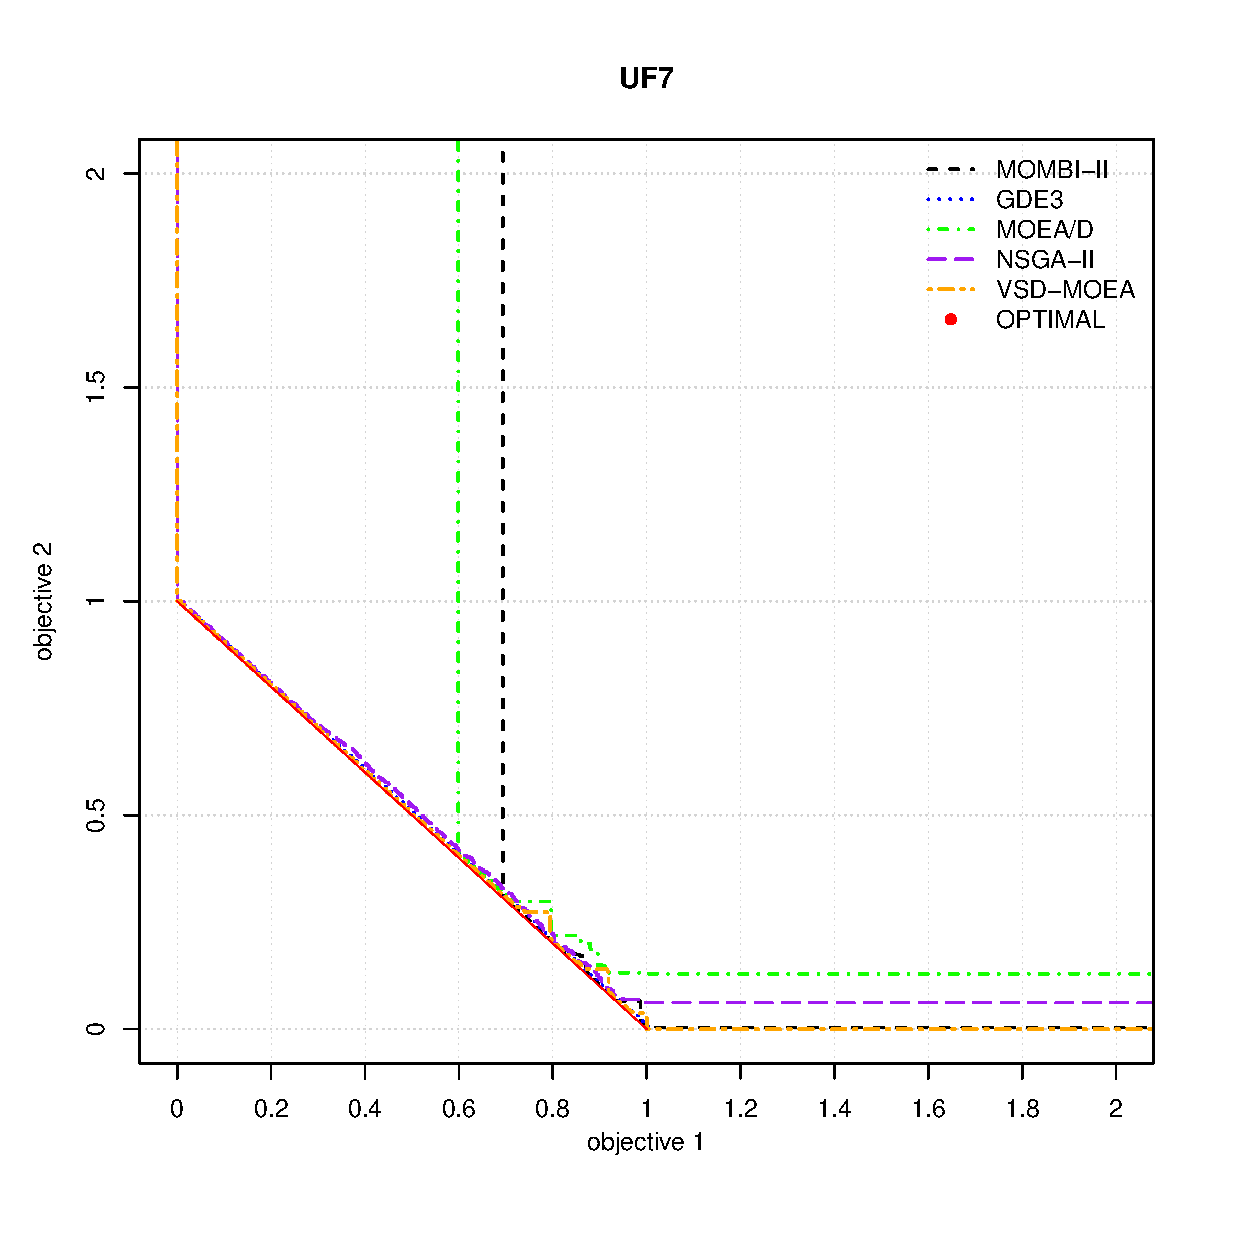
\includegraphics[width=0.33\textwidth]{Surfaces/UF7.eps} &

% \end{tabular}
% \end{figure*}  

% \begin{figure*}
% \centering
% \caption{50\% Attainment Surfaces Achieved}
% \begin{tabular}{ccc}
  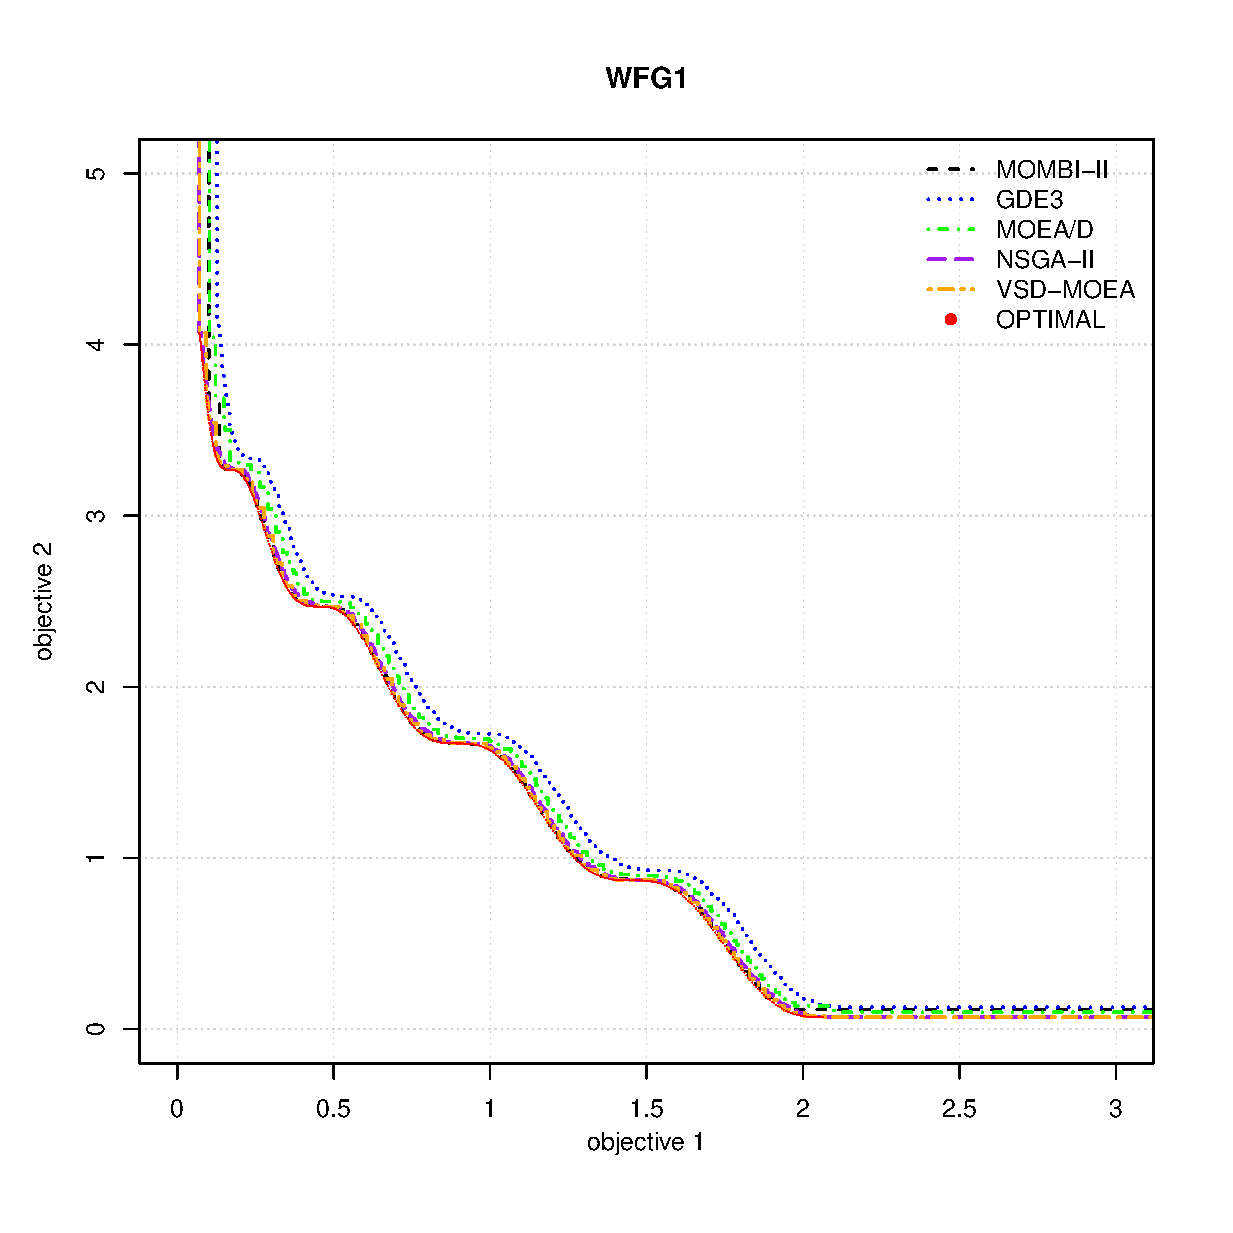
\includegraphics[width=0.33\textwidth]{Surfaces/WFG1.eps} 
  \\
  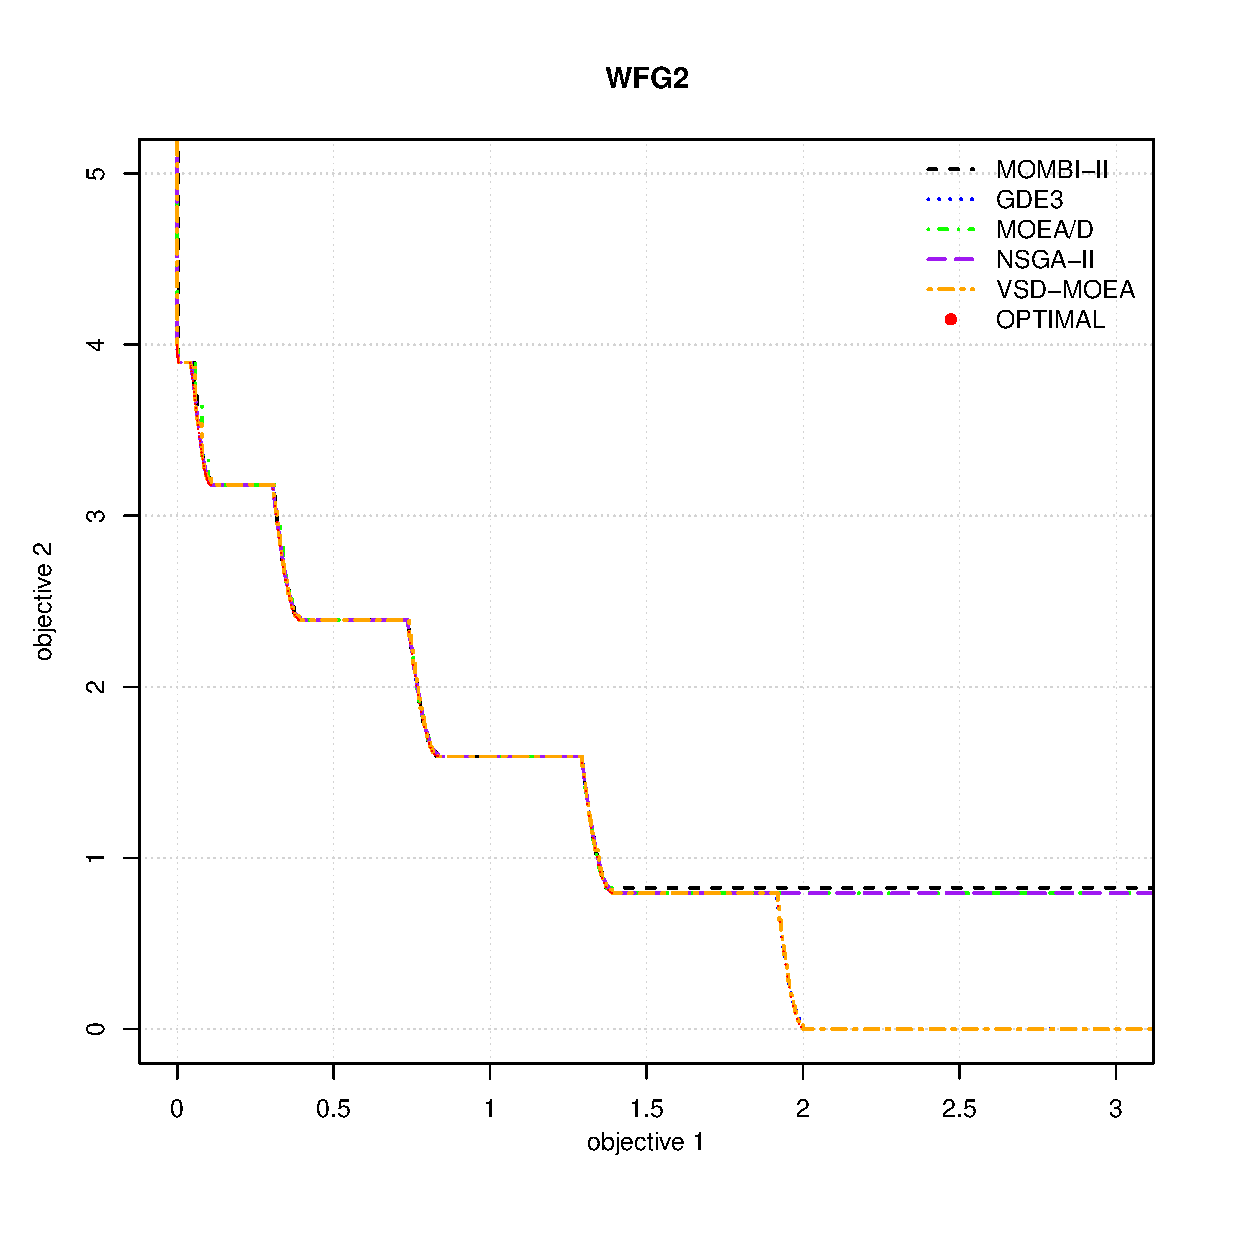
\includegraphics[width=0.33\textwidth]{Surfaces/WFG2.eps} &
%  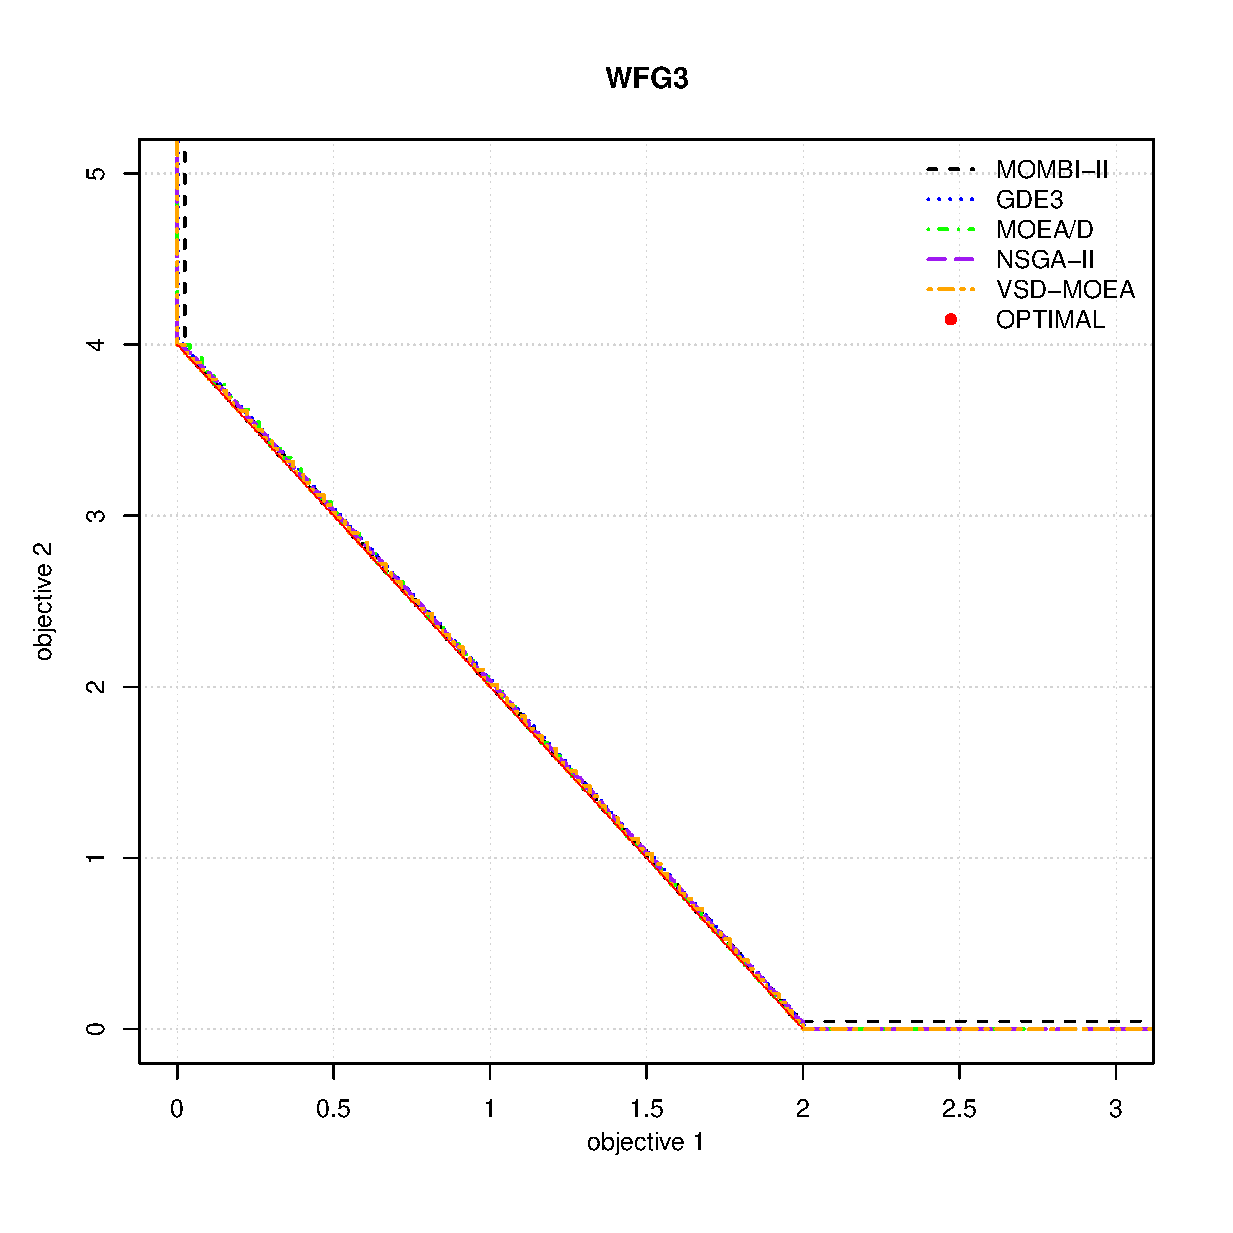
\includegraphics[width=0.33\textwidth]{Surfaces/WFG3.eps} 

  %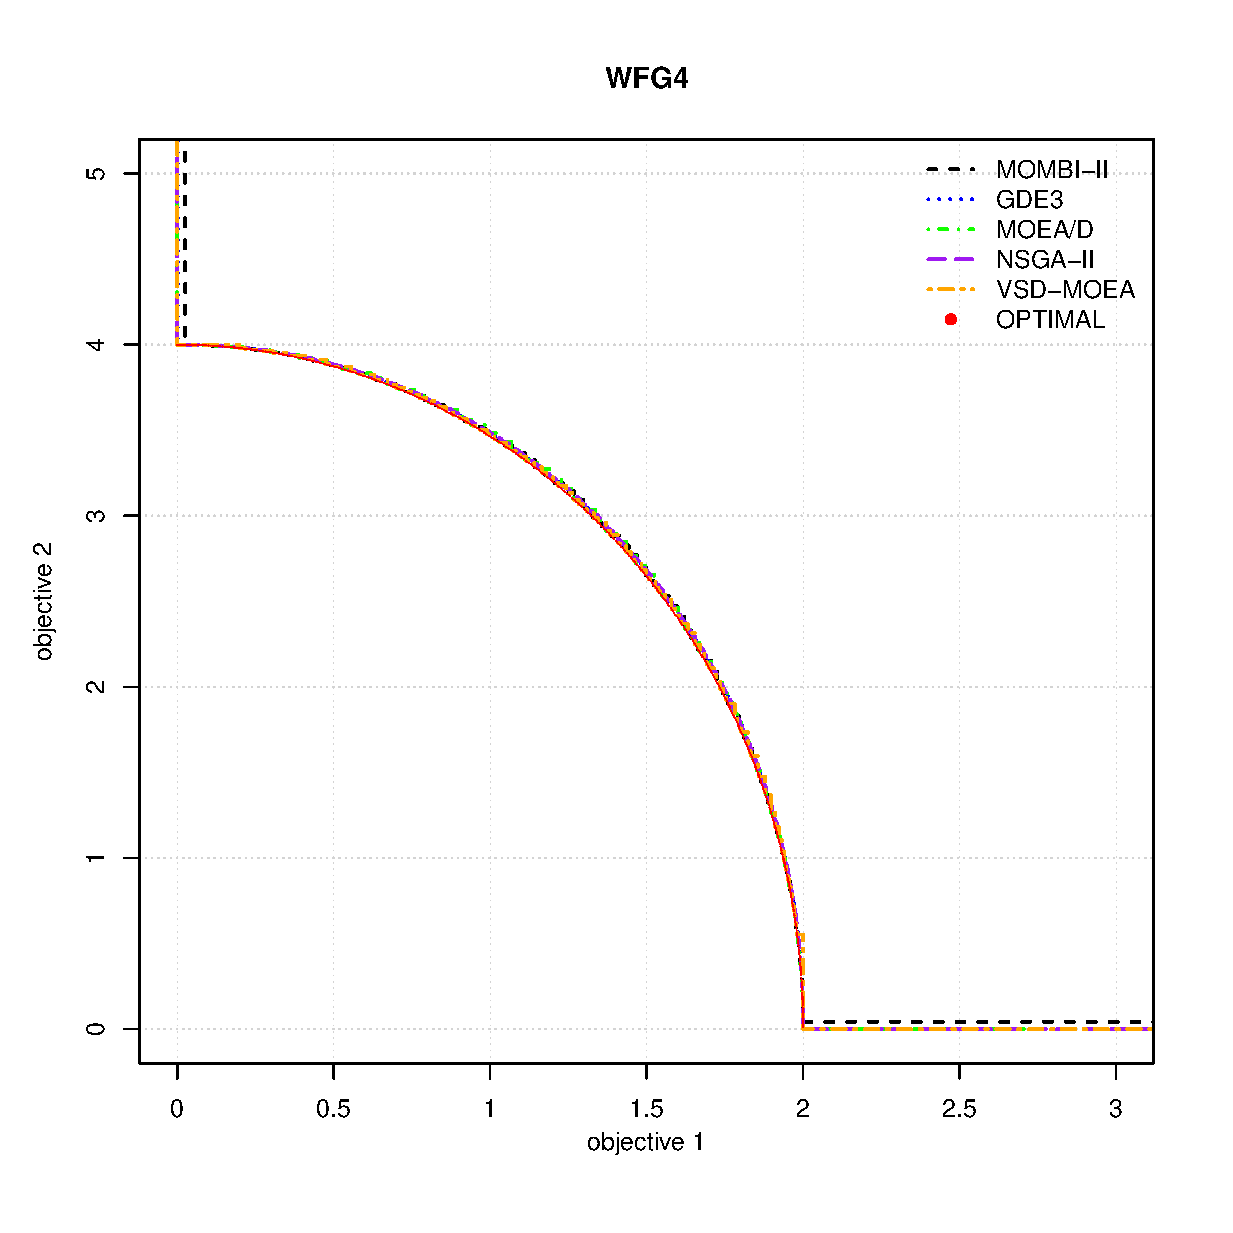
\includegraphics[width=0.33\textwidth]{Surfaces/WFG4.eps} &
  %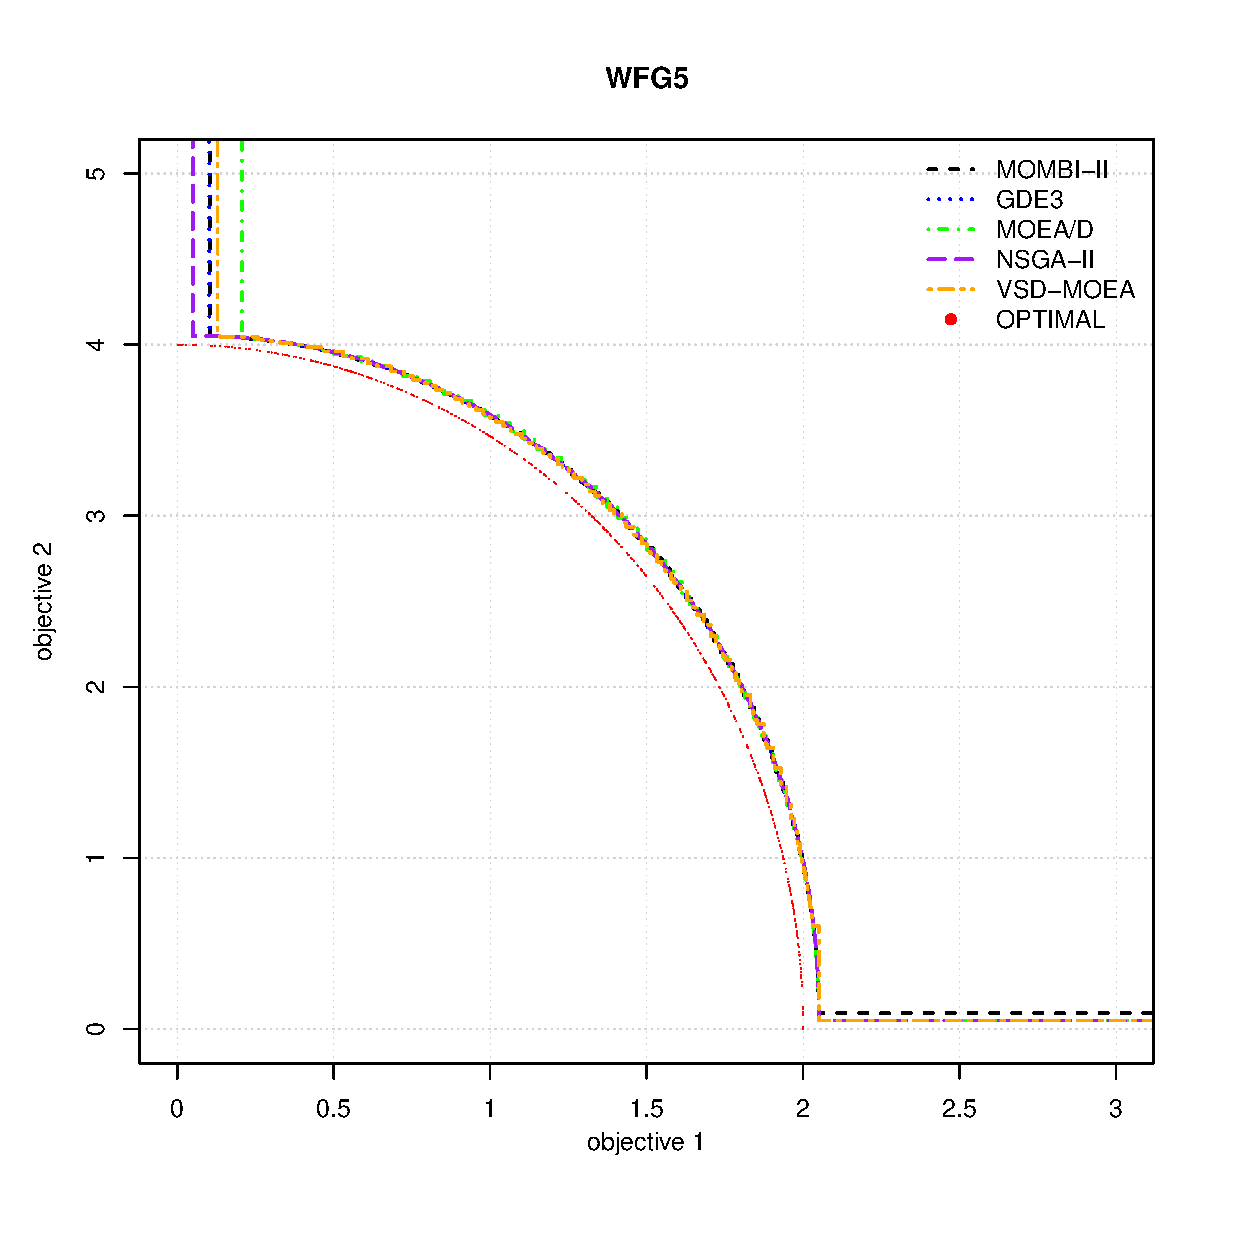
\includegraphics[width=0.33\textwidth]{Surfaces/WFG5.eps} &
  %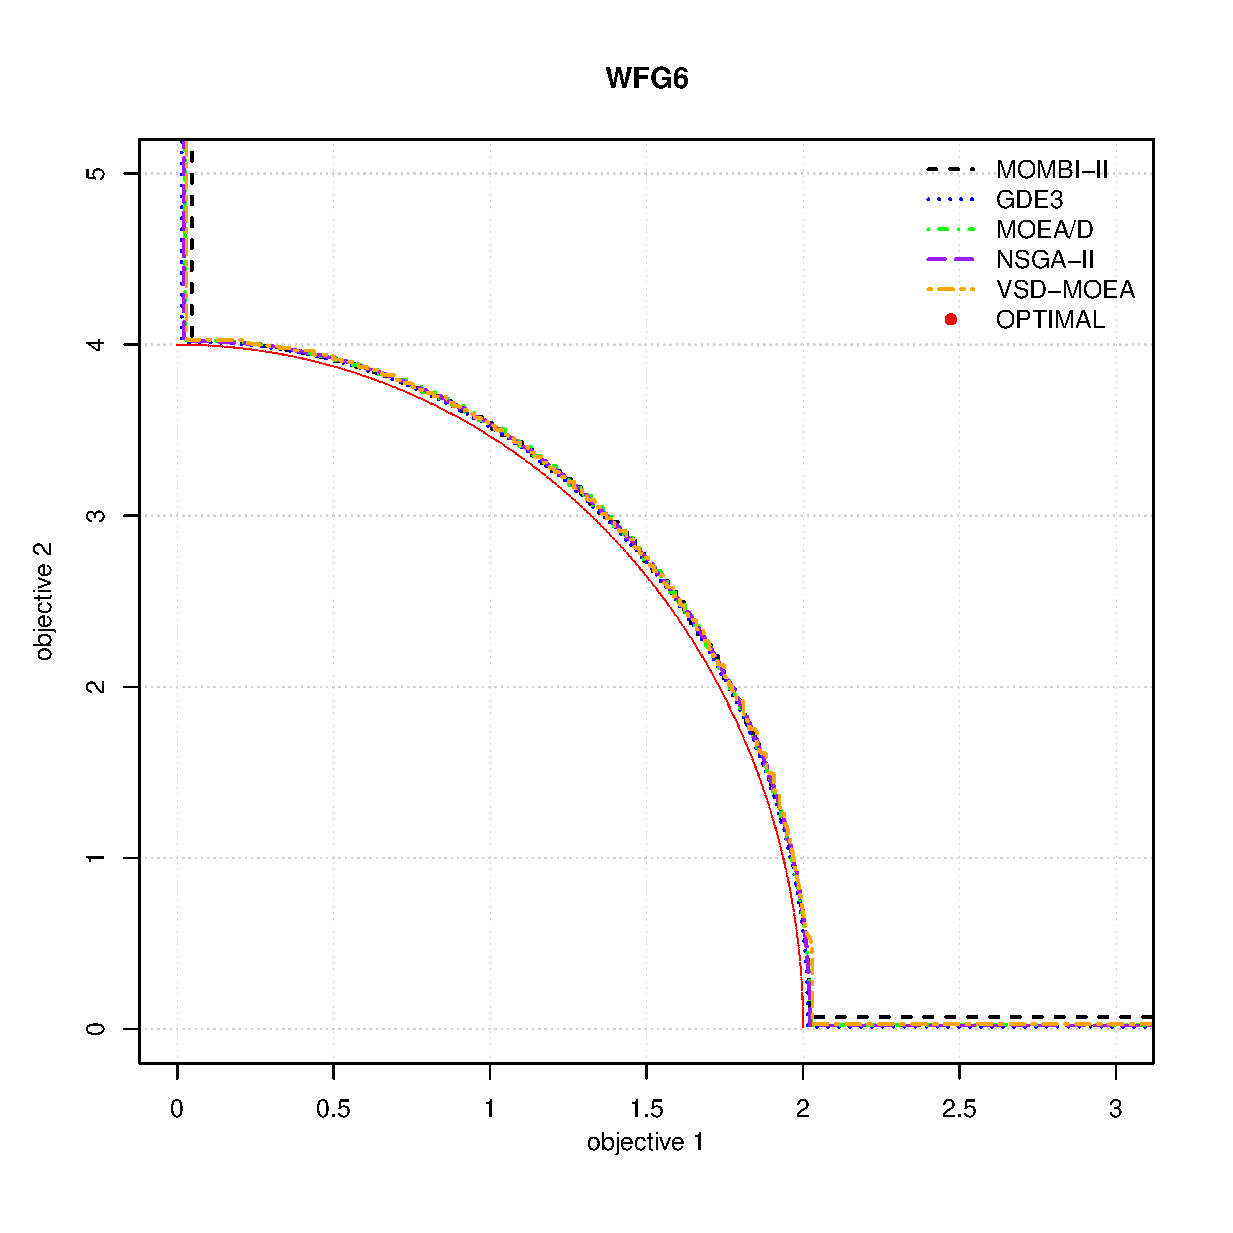
\includegraphics[width=0.33\textwidth]{Surfaces/WFG6.eps} 

  %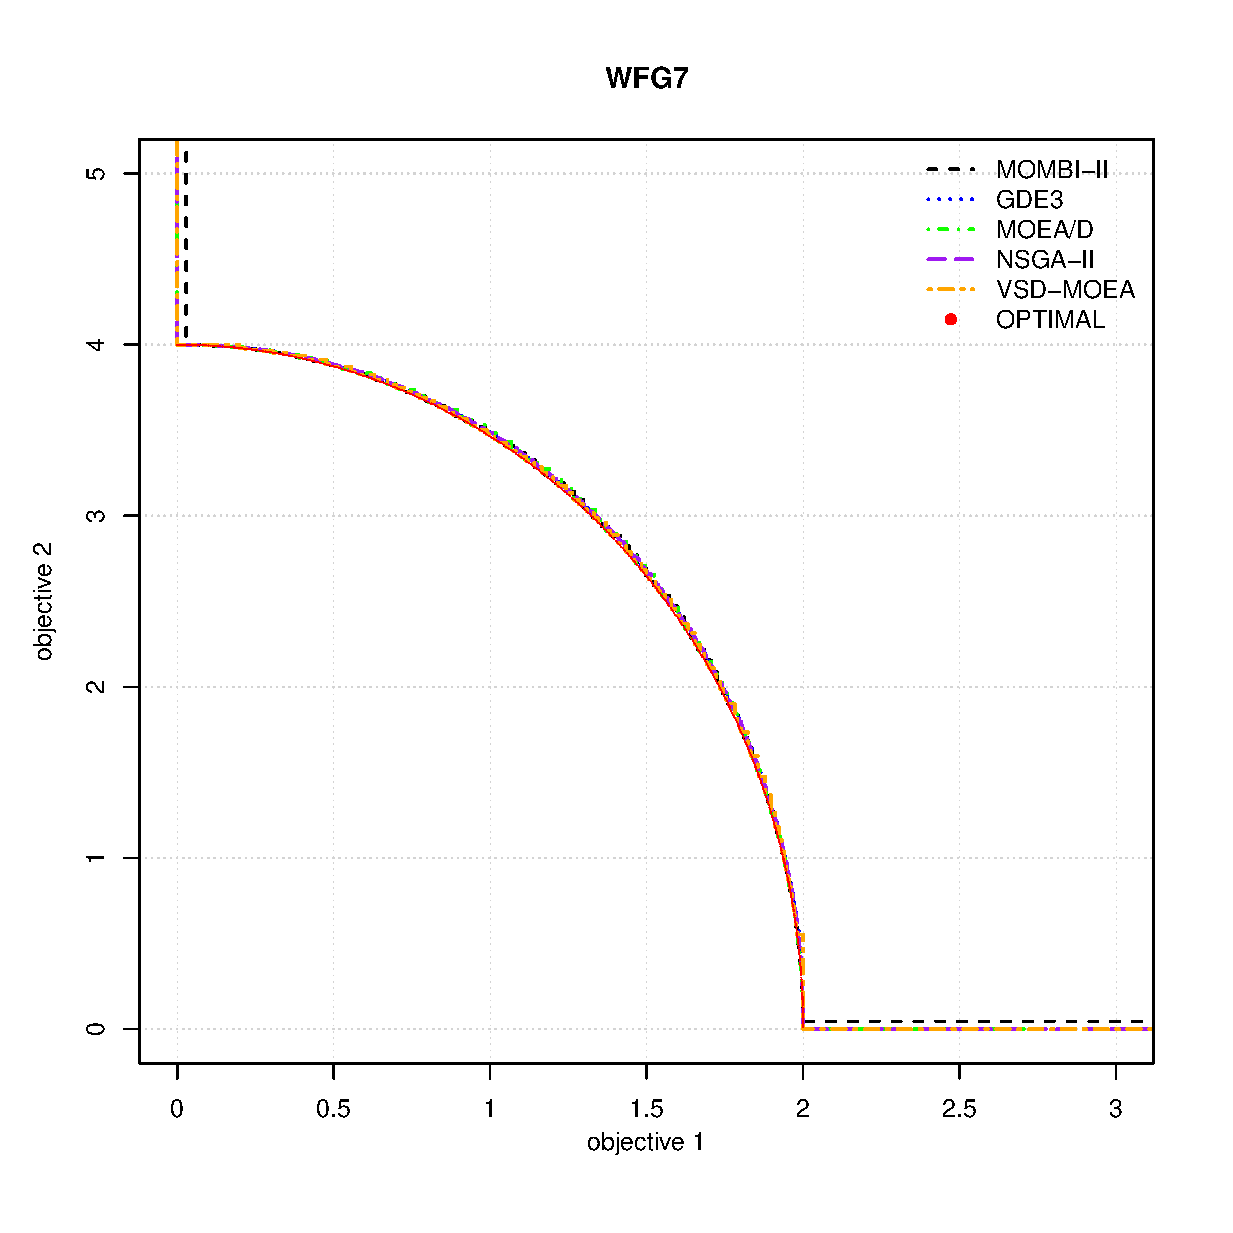
\includegraphics[width=0.33\textwidth]{Surfaces/WFG7.eps} &
  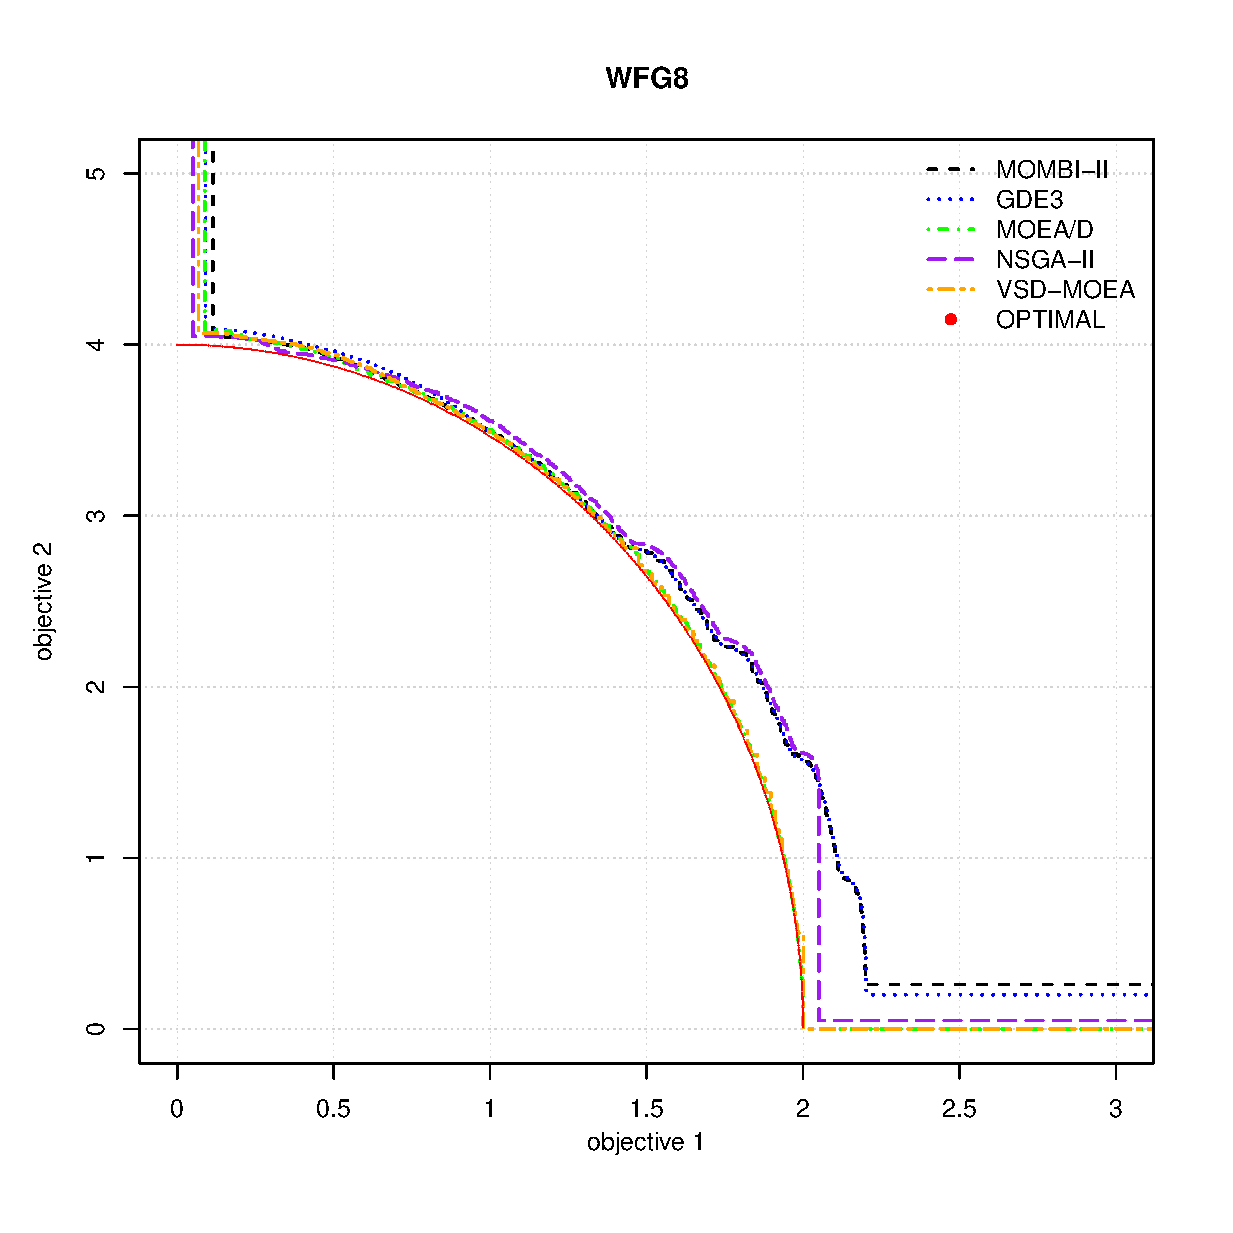
\includegraphics[width=0.33\textwidth]{Surfaces/WFG8.eps} &

  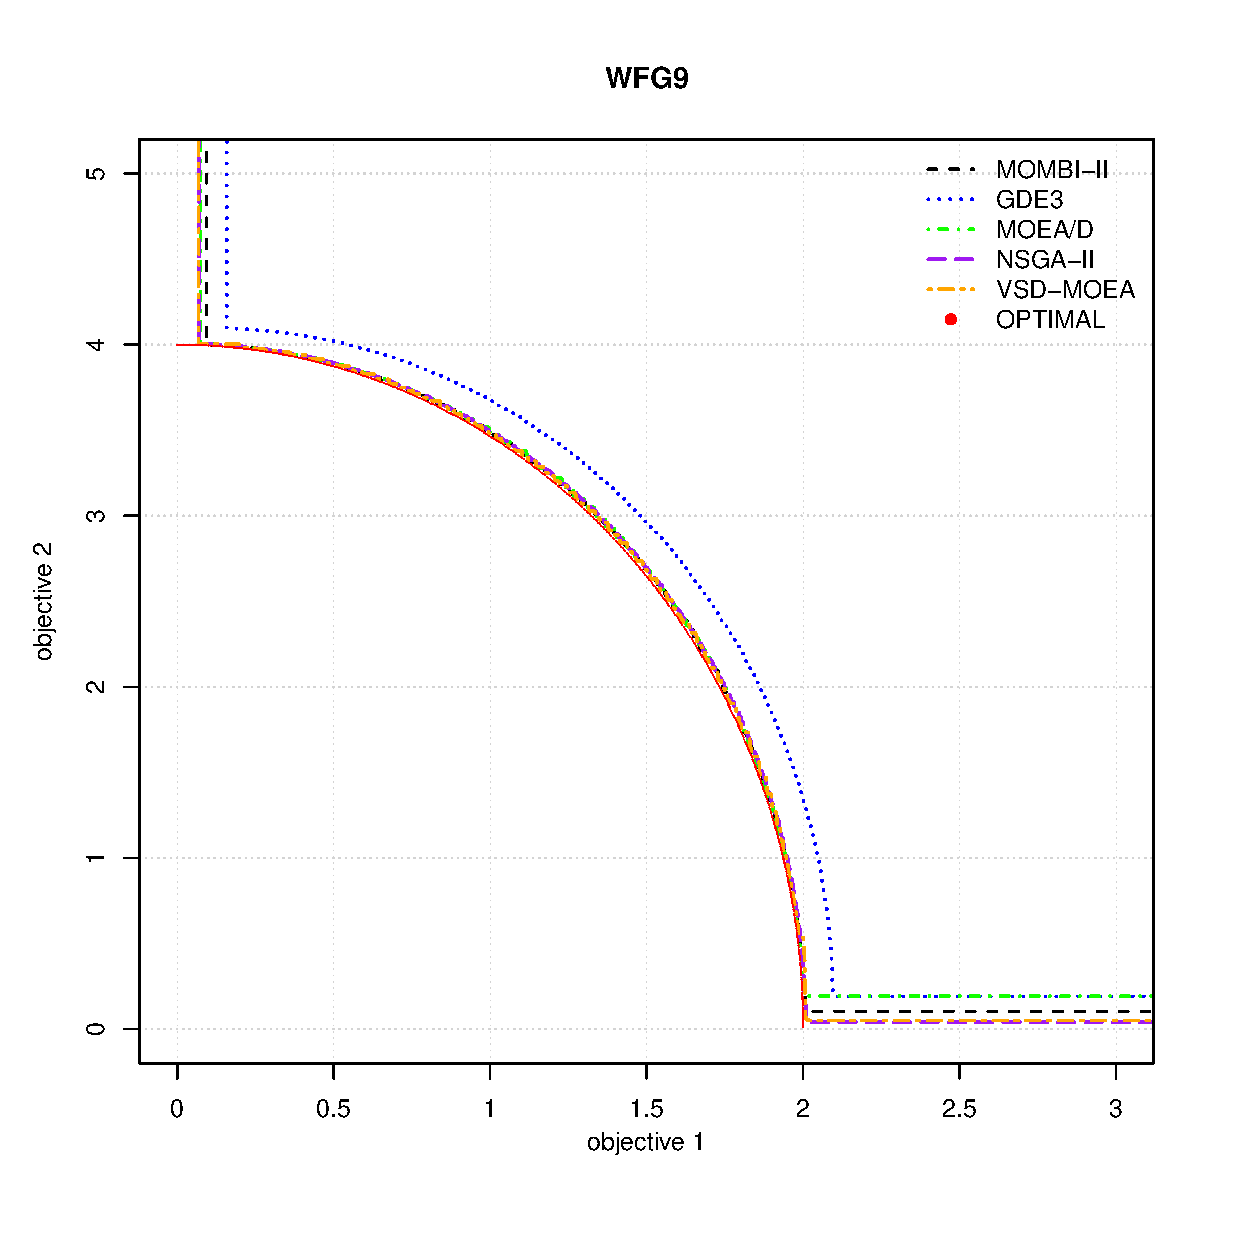
\includegraphics[width=0.33\textwidth]{Surfaces/WFG9.eps}
\end{tabular}
\end{figure*}

%%%%%%%%%%%%%%%%%%%%%%	TABLAS
\begin{table*}[b]
\centering
\caption{Statistics IGD+ with two objectives}
\label{tab:StatisticsHV_2obj}
\resizebox{\textwidth}{!}{%
\begin{tabular}{c|c|c|c|c|c|c|c|c|c|c|c|c|c|c|c|c|c|c|c|c|}
\cline{2-21}
 & \multicolumn{4}{c|}{GDE3} & \multicolumn{4}{c|}{MOMBI-II} & \multicolumn{4}{c|}{NSGAII} & \multicolumn{4}{c|}{MOEA/D} & \multicolumn{4}{c|}{VSD-MOEA} \\ \cline{2-21} 
 & Min & Max & Mean & Diff & Min & Max & Mean & Diff & Min & Max & Mean & Diff & Min & Max & Mean & Diff & Min & Max & Mean & Diff \\ \hline
\multicolumn{1}{|c|}{DTLZ1} & 0.001 & 0.001 & \textbf{0.001} & 0.000 & 0.001 & 0.001 & \textbf{0.001} & 0.000 & 0.002 & 0.002 & 0.002 & 0.000 & 0.001 & 0.001 & \textbf{0.001} & 0.000 & 0.001 & 0.001 & \textbf{0.001} & 0.000 \\ \hline
\multicolumn{1}{|c|}{DTLZ2} & 0.002 & 0.002 & \textbf{0.002} & 0.000 & 0.002 & 0.002 & \textbf{0.002} & 0.000 & 0.002 & 0.003 & 0.003 & 0.001 & 0.002 & 0.002 & \textbf{0.002} & 0.000 & 0.002 & 0.002 & \textbf{0.002} & 0.000 \\ \hline
\multicolumn{1}{|c|}{DTLZ3} & 0.002 & 0.002 & \textbf{0.002} & 0.000 & 0.002 & 0.002 & \textbf{0.002} & 0.000 & 0.002 & 0.003 & 0.003 & 0.001 & 0.002 & 0.002 & 0.002 & 0.000 & 0.002 & 0.002 & \textbf{0.002} & 0.000 \\ \hline
\multicolumn{1}{|c|}{DTLZ4} & 0.002 & 0.002 & \textbf{0.002} & 0.000 & 0.002 & 0.363 & 0.043 & 0.042 & 0.002 & 0.363 & 0.126 & 0.124 & 0.002 & 0.363 & 0.064 & 0.062 & 0.002 & 0.002 & \textbf{0.002} & 0.000 \\ \hline
\multicolumn{1}{|c|}{DTLZ5} & 0.002 & 0.002 & \textbf{0.002} & 0.000 & 0.002 & 0.002 & 0.002 & 0.000 & 0.002 & 0.003 & 0.003 & 0.001 & 0.002 & 0.002 & 0.002 & 0.000 & 0.002 & 0.002 & \textbf{0.002} & 0.000 \\ \hline
\multicolumn{1}{|c|}{DTLZ6} & 0.002 & 0.002 & \textbf{0.002} & 0.000 & 0.002 & 0.108 & 0.059 & 0.057 & 0.003 & 0.089 & 0.051 & 0.049 & 0.002 & 0.110 & 0.067 & 0.065 & 0.002 & 0.132 & 0.054 & 0.052 \\ \hline
\multicolumn{1}{|c|}{DTLZ7} & 0.002 & 0.002 & \textbf{0.002} & 0.000 & 0.363 & 0.363 & 0.363 & 0.361 & 0.361 & 0.361 & 0.361 & 0.359 & 0.361 & 0.361 & 0.361 & 0.359 & 0.003 & 0.003 & 0.003 & 0.001 \\ \hline
\multicolumn{1}{|c|}{UF1} & 0.004 & 0.005 & 0.004 & 0.001 & 0.008 & 0.037 & 0.011 & 0.008 & 0.008 & 0.009 & 0.009 & 0.005 & 0.003 & 0.034 & 0.011 & 0.008 & 0.002 & 0.007 & \textbf{0.003} & 0.000 \\ \hline
\multicolumn{1}{|c|}{UF2} & 0.007 & 0.009 & 0.008 & 0.003 & 0.004 & 0.042 & 0.008 & 0.003 & 0.011 & 0.014 & 0.013 & 0.008 & 0.003 & 0.041 & 0.019 & 0.014 & 0.004 & 0.007 & \textbf{0.005} & 0.000 \\ \hline
\multicolumn{1}{|c|}{UF3} & 0.003 & 0.168 & \textbf{0.013} & 0.000 & 0.017 & 0.046 & 0.030 & 0.017 & 0.015 & 0.034 & 0.024 & 0.011 & 0.007 & 0.196 & 0.037 & 0.024 & 0.028 & 0.058 & 0.040 & 0.027 \\ \hline
\multicolumn{1}{|c|}{UF4} & 0.035 & 0.038 & 0.037 & 0.010 & 0.037 & 0.041 & 0.040 & 0.013 & 0.043 & 0.047 & 0.046 & 0.019 & 0.032 & 0.041 & 0.036 & 0.009 & 0.023 & 0.035 & \textbf{0.027} & 0.000 \\ \hline
\multicolumn{1}{|c|}{UF5} & 0.238 & 0.275 & 0.245 & 0.048 & 0.174 & 0.481 & 0.300 & 0.103 & 0.146 & 0.570 & 0.287 & 0.090 & 0.229 & 0.571 & 0.385 & 0.188 & 0.113 & 0.371 & \textbf{0.197} & 0.000 \\ \hline
\multicolumn{1}{|c|}{UF6} & 0.029 & 0.417 & 0.125 & 0.004 & 0.169 & 0.570 & 0.292 & 0.171 & 0.167 & 0.577 & 0.341 & 0.220 & 0.173 & 1.076 & 0.529 & 0.408 & 0.044 & 0.171 & \textbf{0.121} & 0.000 \\ \hline
\multicolumn{1}{|c|}{UF7} & 0.004 & 0.005 & \textbf{0.004} & 0.000 & 0.004 & 0.254 & 0.230 & 0.226 & 0.008 & 0.385 & 0.083 & 0.079 & 0.003 & 0.492 & 0.194 & 0.189 & 0.004 & 0.013 & 0.005 & 0.001 \\ \hline
\multicolumn{1}{|c|}{WFG1} & 0.005 & 0.214 & 0.088 & 0.073 & 0.000 & 0.137 & 0.029 & 0.014 & 0.006 & 0.113 & 0.024 & 0.009 & 0.008 & 0.166 & 0.049 & 0.034 & 0.006 & 0.115 & \textbf{0.015} & 0.000 \\ \hline
\multicolumn{1}{|c|}{WFG2} & 0.002 & 0.002 & \textbf{0.002} & 0.000 & 0.055 & 0.057 & 0.057 & 0.055 & 0.003 & 0.054 & 0.052 & 0.049 & 0.055 & 0.055 & 0.055 & 0.053 & 0.003 & 0.003 & 0.003 & 0.001 \\ \hline
\multicolumn{1}{|c|}{WFG3} & 0.014 & 0.017 & 0.015 & 0.008 & 0.007 & 0.007 & 0.007 & 0.000 & 0.011 & 0.013 & 0.012 & 0.005 & 0.008 & 0.008 & 0.008 & 0.001 & 0.007 & 0.008 & \textbf{0.007} & 0.000 \\ \hline
\multicolumn{1}{|c|}{WFG4} & 0.007 & 0.008 & 0.007 & 0.001 & 0.006 & 0.006 & 0.006 & 0.000 & 0.007 & 0.009 & 0.008 & 0.002 & 0.007 & 0.007 & 0.007 & 0.001 & 0.006 & 0.006 & \textbf{0.006} & 0.000 \\ \hline
\multicolumn{1}{|c|}{WFG5} & 0.064 & 0.066 & \textbf{0.065} & 0.000 & 0.062 & 0.068 & 0.065 & 0.000 & 0.065 & 0.066 & 0.066 & 0.001 & 0.058 & 0.069 & 0.067 & 0.002 & 0.065 & 0.069 & 0.066 & 0.001 \\ \hline
\multicolumn{1}{|c|}{WFG6} & 0.014 & 0.043 & \textbf{0.025} & 0.000 & 0.020 & 0.050 & 0.032 & 0.007 & 0.021 & 0.049 & 0.034 & 0.008 & 0.024 & 0.073 & 0.037 & 0.011 & 0.022 & 0.045 & 0.035 & 0.010 \\ \hline
\multicolumn{1}{|c|}{WFG7} & 0.008 & 0.009 & 0.008 & 0.002 & 0.006 & 0.006 & 0.006 & 0.000 & 0.007 & 0.009 & 0.008 & 0.003 & 0.007 & 0.007 & 0.007 & 0.001 & 0.006 & 0.006 & \textbf{0.006} & 0.000 \\ \hline
\multicolumn{1}{|c|}{WFG8} & 0.094 & 0.098 & 0.096 & 0.075 & 0.017 & 0.092 & 0.075 & 0.055 & 0.034 & 0.103 & 0.078 & 0.058 & 0.015 & 0.068 & 0.021 & 0.001 & 0.016 & 0.050 & \textbf{0.020} & 0.000 \\ \hline
\multicolumn{1}{|c|}{WFG9} & 0.122 & 0.125 & 0.123 & 0.112 & 0.009 & 0.023 & 0.013 & 0.002 & 0.011 & 0.027 & 0.016 & 0.005 & 0.010 & 0.125 & 0.017 & 0.006 & 0.008 & 0.013 & \textbf{0.011} & 0.000 \\ \hline
\multicolumn{1}{|c|}{Average} & 0.029 & 0.066 & 0.038 & \textbf{0.015} & 0.042 & 0.120 & 0.073 & \textbf{0.049} & 0.041 & 0.126 & 0.072 & \textbf{0.048} & 0.044 & 0.168 & 0.086 & \textbf{0.062} & 0.016 & 0.049 & 0.028 & \textbf{0.004} \\ \hline
\end{tabular}%
}
\end{table*}



% Please add the following required packages to your document preamble:
% \usepackage{graphicx}
\begin{table*}[b]
\centering
\caption{Statistics IGD+ with three objectives}
\label{tab:StatisticsHV_3obj}
\resizebox{\textwidth}{!}{%
\begin{tabular}{c|c|c|c|c|c|c|c|c|c|c|c|c|c|c|c|c|c|c|c|c|}
\cline{2-21}
 & \multicolumn{4}{c|}{GDE3} & \multicolumn{4}{c|}{MOMBI-II} & \multicolumn{4}{c|}{NSGAII} & \multicolumn{4}{c|}{MOEA/D} & \multicolumn{4}{c|}{VSD-MOEA} \\ \cline{2-21} 
 & Min & Max & Mean & Diff & Min & Max & Mean & Diff & Min & Max & Mean & Diff & Min & Max & Mean & Diff & Min & Max & Mean & Diff \\ \hline
\multicolumn{1}{|c|}{DTLZ1} & 0.017 & 0.021 & 0.019 & 0.006 & 0.013 & 0.013 & \textbf{0.013} & 0.000 & 0.018 & 0.023 & 0.020 & 0.007 & 0.014 & 0.014 & 0.014 & 0.001 & 0.013 & 0.015 & 0.014 & 0.001 \\ \hline
\multicolumn{1}{|c|}{DTLZ2} & 0.027 & 0.032 & 0.030 & 0.006 & 0.025 & 0.025 & \textbf{0.025} & 0.000 & 0.028 & 0.036 & 0.032 & 0.007 & 0.028 & 0.028 & 0.028 & 0.004 & 0.023 & 0.025 & 0.024 & 0.000 \\ \hline
\multicolumn{1}{|c|}{DTLZ3} & 0.028 & 0.035 & 0.031 & 0.006 & 0.025 & 0.025 & \textbf{0.025} & 0.000 & 0.028 & 0.037 & 0.031 & 0.007 & 0.028 & 0.028 & 0.028 & 0.004 & 0.024 & 0.024 & 0.024 & 0.000 \\ \hline
\multicolumn{1}{|c|}{DTLZ4} & 0.028 & 0.033 & 0.030 & 0.006 & 0.025 & 0.364 & 0.042 & 0.018 & 0.028 & 0.595 & 0.046 & 0.022 & 0.028 & 0.595 & 0.107 & 0.082 & 0.024 & 0.024 & \textbf{0.024} & 0.000 \\ \hline
\multicolumn{1}{|c|}{DTLZ5} & 0.002 & 0.002 & \textbf{0.002} & 0.000 & 0.004 & 0.004 & 0.004 & 0.002 & 0.003 & 0.003 & 0.003 & 0.001 & 0.003 & 0.003 & 0.003 & 0.001 & 0.002 & 0.002 & \textbf{0.002} & 0.000 \\ \hline
\multicolumn{1}{|c|}{DTLZ6} & 0.002 & 0.002 & \textbf{0.002} & 0.000 & 0.004 & 0.125 & 0.065 & 0.064 & 0.003 & 0.072 & 0.041 & 0.039 & 0.045 & 0.159 & 0.094 & 0.092 & 0.002 & 0.124 & 0.060 & 0.058 \\ \hline
\multicolumn{1}{|c|}{DTLZ7} & 0.031 & 0.043 & 0.035 & 0.007 & 0.688 & 0.689 & 0.689 & 0.661 & 0.683 & 0.684 & 0.683 & 0.655 & 0.685 & 0.685 & 0.685 & 0.657 & 0.027 & 0.029 & \textbf{0.028} & 0.000 \\ \hline
\multicolumn{1}{|c|}{UF10} & 0.609 & 2.740 & 1.545 & 1.444 & 0.182 & 0.473 & 0.339 & 0.237 & 0.178 & 0.388 & 0.308 & 0.207 & 0.326 & 0.478 & 0.389 & 0.288 & 0.075 & 0.225 & \textbf{0.101} & 0.000 \\ \hline
\multicolumn{1}{|c|}{UF8} & 0.442 & 2.747 & 1.259 & 1.225 & 0.035 & 0.365 & 0.098 & 0.064 & 0.071 & 0.089 & 0.078 & 0.044 & 0.035 & 0.365 & 0.137 & 0.103 & 0.025 & 0.060 & \textbf{0.034} & 0.000 \\ \hline
\multicolumn{1}{|c|}{UF9} & 0.701 & 2.225 & 1.345 & 1.318 & 0.025 & 0.143 & 0.113 & 0.086 & 0.073 & 0.229 & 0.128 & 0.101 & 0.034 & 0.143 & 0.124 & 0.098 & 0.023 & 0.033 & \textbf{0.027} & 0.000 \\ \hline
\multicolumn{1}{|c|}{WFG1} & 1.169 & 1.276 & 1.236 & 1.172 & 0.008 & 0.224 & 0.064 & 0.000 & 0.123 & 0.168 & 0.141 & 0.077 & 0.080 & 0.209 & 0.122 & 0.058 & 0.052 & 0.099 & \textbf{0.064} & 0.000 \\ \hline
\multicolumn{1}{|c|}{WFG2} & 0.092 & 0.149 & 0.118 & 0.078 & 0.040 & 0.108 & 0.066 & 0.027 & 0.095 & 0.168 & 0.140 & 0.101 & 0.044 & 0.117 & 0.087 & 0.047 & 0.031 & 0.055 & \textbf{0.040} & 0.000 \\ \hline
\multicolumn{1}{|c|}{WFG3} & 0.046 & 0.094 & 0.066 & 0.041 & 0.024 & 0.027 & 0.026 & 0.002 & 0.032 & 0.074 & 0.047 & 0.023 & 0.024 & 0.025 & \textbf{0.025} & 0.000 & 0.036 & 0.039 & 0.037 & 0.012 \\ \hline
\multicolumn{1}{|c|}{WFG4} & 0.192 & 0.245 & 0.214 & 0.128 & 0.085 & 0.085 & \textbf{0.085} & 0.000 & 0.113 & 0.135 & 0.123 & 0.037 & 0.122 & 0.126 & 0.124 & 0.039 & 0.084 & 0.093 & 0.089 & 0.003 \\ \hline
\multicolumn{1}{|c|}{WFG5} & 0.151 & 0.171 & 0.159 & 0.014 & 0.144 & 0.145 & \textbf{0.145} & 0.000 & 0.160 & 0.177 & 0.167 & 0.022 & 0.176 & 0.185 & 0.180 & 0.035 & 0.141 & 0.152 & 0.147 & 0.002 \\ \hline
\multicolumn{1}{|c|}{WFG6} & 0.182 & 0.263 & 0.220 & 0.109 & 0.101 & 0.128 & \textbf{0.110} & 0.000 & 0.134 & 0.191 & 0.155 & 0.044 & 0.143 & 0.176 & 0.154 & 0.044 & 0.103 & 0.130 & 0.114 & 0.004 \\ \hline
\multicolumn{1}{|c|}{WFG7} & 0.174 & 0.218 & 0.197 & 0.112 & 0.085 & 0.085 & \textbf{0.085} & 0.000 & 0.107 & 0.134 & 0.120 & 0.035 & 0.126 & 0.126 & 0.126 & 0.041 & 0.084 & 0.094 & 0.089 & 0.003 \\ \hline
\multicolumn{1}{|c|}{WFG8} & 0.310 & 0.352 & 0.331 & 0.227 & 0.092 & 0.147 & \textbf{0.104} & 0.000 & 0.216 & 0.265 & 0.232 & 0.129 & 0.132 & 0.143 & 0.136 & 0.032 & 0.091 & 0.226 & 0.114 & 0.010 \\ \hline
\multicolumn{1}{|c|}{WFG9} & 0.223 & 0.247 & 0.235 & 0.135 & 0.090 & 0.208 & \textbf{0.100} & 0.000 & 0.131 & 0.250 & 0.229 & 0.130 & 0.129 & 0.241 & 0.139 & 0.040 & 0.090 & 0.208 & 0.104 & 0.004 \\ \hline
\multicolumn{1}{|c|}{Average} & 0.233 & 0.573 & 0.372 & \textbf{0.318} & 0.089 & 0.178 & 0.116 & \textbf{0.061} & 0.117 & 0.196 & 0.143 & \textbf{0.089} & 0.116 & 0.202 & 0.142 & \textbf{0.088} & 0.050 & 0.087 & 0.060 & \textbf{0.005} \\ \hline
\end{tabular}%
}
\end{table*}



% Please add the following required packages to your document preamble:
% \usepackage{graphicx}
\begin{table*}[b]
\centering
\caption{Effective tests IGD+ with two objectives}
\label{tab:Effective_Test_2obj}
\resizebox{\textwidth}{!}{%
\begin{tabular}{|c|c|c|c|c|c|c|c|c|c|c|c|c|c|c|c|}
\hline
 & \multicolumn{3}{c|}{GDE3} & \multicolumn{3}{c|}{MOMBI2} & \multicolumn{3}{c|}{NSGA-II} & \multicolumn{3}{c|}{MOEA/D} & \multicolumn{3}{c|}{VSD-MOEA} \\ \hline
 & $\uparrow$ & $\downarrow$ & Score & $\uparrow$ & $\downarrow$ & Score & $\uparrow$ & $\downarrow$ & Score & $\uparrow$ & $\downarrow$ & Score & $\uparrow$ & $\downarrow$ & Score \\ \hline
DTLZ1 & 0.001 & 0.000 & 0.000 & 0.001 & 0.000 & \textbf{0.001} & 0.000 & 0.002 & -0.002 & 0.001 & 0.000 & \textbf{0.001} & 0.000 & 0.000 & 0.000 \\ \hline
DTLZ2 & 0.001 & 0.000 & \textbf{0.001} & 0.000 & 0.000 & 0.000 & 0.000 & 0.002 & -0.002 & 0.001 & 0.000 & 0.000 & 0.001 & 0.000 & 0.000 \\ \hline
DTLZ3 & 0.001 & 0.000 & \textbf{0.001} & 0.000 & 0.000 & 0.000 & 0.000 & 0.002 & -0.002 & 0.000 & 0.000 & 0.000 & 0.001 & 0.000 & 0.000 \\ \hline
DTLZ4 & 0.228 & 0.000 & \textbf{0.228} & 0.104 & 0.083 & 0.021 & 0.000 & 0.394 & -0.394 & 0.062 & 0.145 & -0.083 & 0.228 & 0.000 & 0.227 \\ \hline
DTLZ5 & 0.001 & 0.000 & \textbf{0.001} & 0.000 & 0.000 & 0.000 & 0.000 & 0.002 & -0.002 & 0.001 & 0.000 & 0.000 & 0.001 & 0.000 & 0.000 \\ \hline
DTLZ6 & 0.223 & 0.000 & \textbf{0.223} & 0.000 & 0.057 & -0.057 & 0.016 & 0.049 & -0.032 & 0.000 & 0.094 & -0.094 & 0.013 & 0.052 & -0.039 \\ \hline
DTLZ7 & 1.080 & 0.000 & \textbf{1.080} & 0.000 & 0.725 & -0.725 & 0.002 & 0.718 & -0.716 & 0.002 & 0.718 & -0.716 & 1.077 & 0.001 & 1.077 \\ \hline
UF1 & 0.019 & 0.001 & 0.018 & 0.000 & 0.018 & -0.018 & 0.006 & 0.010 & -0.004 & 0.000 & 0.018 & -0.018 & 0.022 & 0.000 & \textbf{0.022} \\ \hline
UF2 & 0.016 & 0.003 & 0.013 & 0.016 & 0.000 & 0.016 & 0.006 & 0.018 & -0.012 & 0.000 & 0.040 & -0.040 & 0.024 & 0.000 & \textbf{0.024} \\ \hline
UF3 & 0.079 & 0.000 & \textbf{0.079} & 0.011 & 0.023 & -0.012 & 0.023 & 0.011 & 0.012 & 0.003 & 0.024 & -0.021 & 0.000 & 0.058 & -0.058 \\ \hline
UF4 & 0.011 & 0.012 & -0.001 & 0.006 & 0.020 & -0.013 & 0.000 & 0.044 & -0.044 & 0.016 & 0.009 & 0.007 & 0.052 & 0.000 & \textbf{0.052} \\ \hline
UF5 & 0.237 & 0.048 & 0.189 & 0.085 & 0.158 & -0.073 & 0.098 & 0.132 & -0.033 & 0.000 & 0.512 & -0.512 & 0.429 & 0.000 & \textbf{0.429} \\ \hline
UF6 & 0.787 & 0.000 & 0.787 & 0.286 & 0.338 & -0.052 & 0.188 & 0.485 & -0.297 & 0.000 & 1.238 & -1.238 & 0.800 & 0.000 & \textbf{0.800} \\ \hline
UF7 & 0.494 & 0.000 & \textbf{0.494} & 0.000 & 0.597 & -0.597 & 0.257 & 0.157 & 0.100 & 0.000 & 0.488 & -0.488 & 0.491 & 0.000 & 0.491 \\ \hline
WFG1 & 0.000 & 0.234 & -0.234 & 0.079 & 0.000 & 0.079 & 0.089 & 0.009 & 0.080 & 0.039 & 0.078 & -0.039 & 0.115 & 0.000 & \textbf{0.115} \\ \hline
WFG2 & 0.158 & 0.000 & \textbf{0.158} & 0.000 & 0.116 & -0.116 & 0.009 & 0.098 & -0.089 & 0.002 & 0.109 & -0.107 & 0.155 & 0.001 & 0.155 \\ \hline
WFG3 & 0.000 & 0.026 & -0.026 & 0.015 & 0.000 & \textbf{0.015} & 0.003 & 0.014 & -0.011 & 0.011 & 0.001 & 0.010 & 0.013 & 0.000 & 0.012 \\ \hline
WFG4 & 0.001 & 0.003 & -0.002 & 0.004 & 0.000 & \textbf{0.004} & 0.000 & 0.007 & -0.007 & 0.002 & 0.001 & 0.001 & 0.004 & 0.000 & \textbf{0.004} \\ \hline
WFG5 & 0.005 & 0.000 & \textbf{0.005} & 0.003 & 0.000 & 0.003 & 0.001 & 0.002 & 0.000 & 0.000 & 0.007 & -0.007 & 0.001 & 0.002 & -0.001 \\ \hline
WFG6 & 0.037 & 0.000 & \textbf{0.037} & 0.000 & 0.007 & -0.007 & 0.000 & 0.008 & -0.008 & 0.000 & 0.011 & -0.011 & 0.000 & 0.010 & -0.010 \\ \hline
WFG7 & 0.000 & 0.007 & -0.007 & 0.006 & 0.000 & \textbf{0.006} & 0.000 & 0.007 & -0.007 & 0.004 & 0.001 & 0.002 & 0.006 & 0.000 & \textbf{0.006} \\ \hline
WFG8 & 0.000 & 0.188 & -0.188 & 0.020 & 0.110 & -0.089 & 0.018 & 0.115 & -0.097 & 0.186 & 0.000 & 0.186 & 0.188 & 0.000 & \textbf{0.188} \\ \hline
WFG9 & 0.000 & 0.436 & -0.436 & 0.112 & 0.002 & 0.110 & 0.109 & 0.007 & 0.102 & 0.106 & 0.008 & 0.098 & 0.126 & 0.000 & \textbf{0.126} \\ \hline
Total & 3.378 & 0.958 & \textbf{2.420} & 0.749 & 2.256 & \textbf{-1.507} & 0.824 & 2.290 & \textbf{-1.466} & 0.435 & 3.505 & \textbf{-3.070} & 3.747 & 0.124 & \textbf{3.622} \\ \hline
\end{tabular}%
}
\end{table*}


% Please add the following required packages to your document preamble:
% \usepackage{graphicx}
\begin{table*}[b]
\centering
\caption{Effective tests IGD+ with three objectives}
\label{tab:Effective_Test_3obj}
\resizebox{\textwidth}{!}{%
\begin{tabular}{|c|c|c|c|c|c|c|c|c|c|c|c|c|c|c|c|}
\hline
 & \multicolumn{3}{c|}{GDE3} & \multicolumn{3}{c|}{MOMBI2} & \multicolumn{3}{c|}{NSGA-II} & \multicolumn{3}{c|}{MOEA/D} & \multicolumn{3}{c|}{VSD-MOEA} \\ \hline
 & $\uparrow$ & $\downarrow$ & Score & $\uparrow$ & $\downarrow$ & Score & $\uparrow$ & $\downarrow$ & Score & $\uparrow$ & $\downarrow$ & Score & $\uparrow$ & $\downarrow$ & Score \\ \hline
DTLZ1 & 0.001 & 0.015 & -0.015 & 0.015 & 0.000 & \textbf{0.015} & 0.000 & 0.019 & -0.019 & 0.010 & 0.002 & 0.008 & 0.011 & 0.001 & 0.010 \\ \hline
DTLZ2 & 0.001 & 0.014 & -0.013 & 0.016 & 0.000 & 0.016 & 0.000 & 0.020 & -0.020 & 0.006 & 0.007 & -0.001 & 0.017 & 0.000 & \textbf{0.017} \\ \hline
DTLZ3 & 0.000 & 0.015 & -0.015 & 0.016 & 0.000 & 0.016 & 0.000 & 0.018 & -0.018 & 0.006 & 0.007 & -0.001 & 0.018 & 0.000 & \textbf{0.018} \\ \hline
DTLZ4 & 0.012 & 0.006 & 0.006 & 0.069 & 0.029 & 0.040 & 0.060 & 0.026 & 0.034 & 0.000 & 0.208 & -0.208 & 0.128 & 0.000 & \textbf{0.128} \\ \hline
DTLZ5 & 0.004 & 0.000 & \textbf{0.004} & 0.000 & 0.004 & -0.004 & 0.001 & 0.002 & 0.000 & 0.000 & 0.003 & -0.003 & 0.004 & 0.000 & 0.003 \\ \hline
DTLZ6 & 0.253 & 0.000 & \textbf{0.253} & 0.028 & 0.088 & -0.060 & 0.097 & 0.039 & 0.059 & 0.000 & 0.206 & -0.206 & 0.033 & 0.078 & -0.045 \\ \hline
DTLZ7 & 1.954 & 0.007 & 1.947 & 0.000 & 1.326 & -1.326 & 0.008 & 1.304 & -1.295 & 0.004 & 1.310 & -1.306 & 1.980 & 0.000 & \textbf{1.980} \\ \hline
UF10 & 0.000 & 5.043 & -5.043 & 1.207 & 0.237 & 0.969 & 1.318 & 0.207 & 1.111 & 1.156 & 0.368 & 0.788 & 2.175 & 0.000 & \textbf{2.175} \\ \hline
UF8 & 0.000 & 4.688 & -4.688 & 1.161 & 0.083 & 1.078 & 1.260 & 0.044 & 1.216 & 1.121 & 0.163 & 0.959 & 1.435 & 0.000 & \textbf{1.435} \\ \hline
UF9 & 0.000 & 4.989 & -4.989 & 1.244 & 0.086 & 1.158 & 1.217 & 0.101 & 1.116 & 1.221 & 0.109 & 1.111 & 1.603 & 0.000 & \textbf{1.603} \\ \hline
WFG1 & 0.000 & 4.551 & -4.551 & 1.307 & 0.000 & \textbf{1.307} & 1.095 & 0.173 & 0.922 & 1.132 & 0.117 & 1.015 & 1.307 & 0.000 & \textbf{1.307} \\ \hline
WFG2 & 0.023 & 0.160 & -0.137 & 0.146 & 0.027 & 0.119 & 0.000 & 0.251 & -0.251 & 0.085 & 0.067 & 0.018 & 0.252 & 0.000 & \textbf{0.252} \\ \hline
WFG3 & 0.000 & 0.127 & -0.127 & 0.071 & 0.002 & 0.069 & 0.018 & 0.054 & -0.036 & 0.078 & 0.000 & \textbf{0.078} & 0.039 & 0.023 & 0.016 \\ \hline
WFG4 & 0.000 & 0.434 & -0.434 & 0.208 & 0.000 & \textbf{0.208} & 0.091 & 0.071 & 0.019 & 0.089 & 0.075 & 0.015 & 0.195 & 0.003 & 0.191 \\ \hline
WFG5 & 0.029 & 0.026 & 0.003 & 0.074 & 0.000 & \textbf{0.074} & 0.013 & 0.051 & -0.038 & 0.000 & 0.102 & -0.102 & 0.065 & 0.002 & 0.062 \\ \hline
WFG6 & 0.000 & 0.346 & -0.346 & 0.202 & 0.000 & \textbf{0.202} & 0.065 & 0.085 & -0.020 & 0.065 & 0.084 & -0.019 & 0.187 & 0.004 & 0.183 \\ \hline
WFG7 & 0.000 & 0.369 & -0.369 & 0.190 & 0.000 & \textbf{0.190} & 0.083 & 0.066 & 0.017 & 0.071 & 0.084 & -0.013 & 0.178 & 0.003 & 0.175 \\ \hline
WFG8 & 0.000 & 0.737 & -0.737 & 0.388 & 0.000 & \textbf{0.388} & 0.098 & 0.344 & -0.245 & 0.292 & 0.053 & 0.239 & 0.356 & 0.000 & 0.356 \\ \hline
WFG9 & 0.000 & 0.361 & -0.361 & 0.304 & 0.000 & \textbf{0.304} & 0.000 & 0.345 & -0.345 & 0.185 & 0.075 & 0.110 & 0.291 & 0.000 & 0.291 \\ \hline
Total & 2.277 & 21.888 & \textbf{-19.612} & 6.647 & 1.883 & \textbf{4.763} & 5.425 & 3.219 & \textbf{2.206} & 5.523 & 3.040 & \textbf{2.482} & 10.274 & 0.115 & \textbf{10.160} \\ \hline
\end{tabular}%
}
\end{table*}


